\chapter{Resultados}
\label{CAP::Resultados}
Se presentan cuatro casos de ejecución desde la interfaz y, después, los cuatro experimentos que miden el método. Los tres primeros casos resuelven problemas con mallas, estados iniciales, metas y perfiles distintos; el cuarto muestra cómo el sistema detecta una meta imposible. Todos los tiempos se midieron en un equipo con procesador Intel Core i5-13420H, 16 GB de memoria y Node 22.

\section{Caso 1: Ana Ruiz, alumna irregular}

\subsection{Descripción}
Ana Ruiz estudia Ingeniería en Desarrollo de Software (ISW). Aprobó siete materias de los dos primeros niveles, reprobó Cálculo diferencial (ISW01) y su siguiente inscripción es en mayo. Quiere saber en cuántos cuatrimestres termina la carrera con la especialidad A si lleva la carga regular. El caso no es trivial porque Cálculo diferencial encabeza la cadena más larga que le falta, ISW01 $\to$ ISW06 $\to$ ISW12 $\to$ ISW28, y varias materias de los niveles 3 a 5 solo se abren en dos periodos.

\subsection{Estado inicial y meta}
El estado inicial es $(A_0, \text{May})$ con $A_0 = \{$ISW02, ISW03, ISW04, ISW05, ISW07, ISW08, ISW09$\}$. La Figura~\ref{FIG::C1Historial} muestra la pantalla de historial: ISW01 aparece como reprobada, las materias disponibles en mayo tienen borde punteado y el panel derecho muestra $A_0$, $p_0$ y la cota inicial $h = 4$.

\begin{figure}[H]
    \centering
    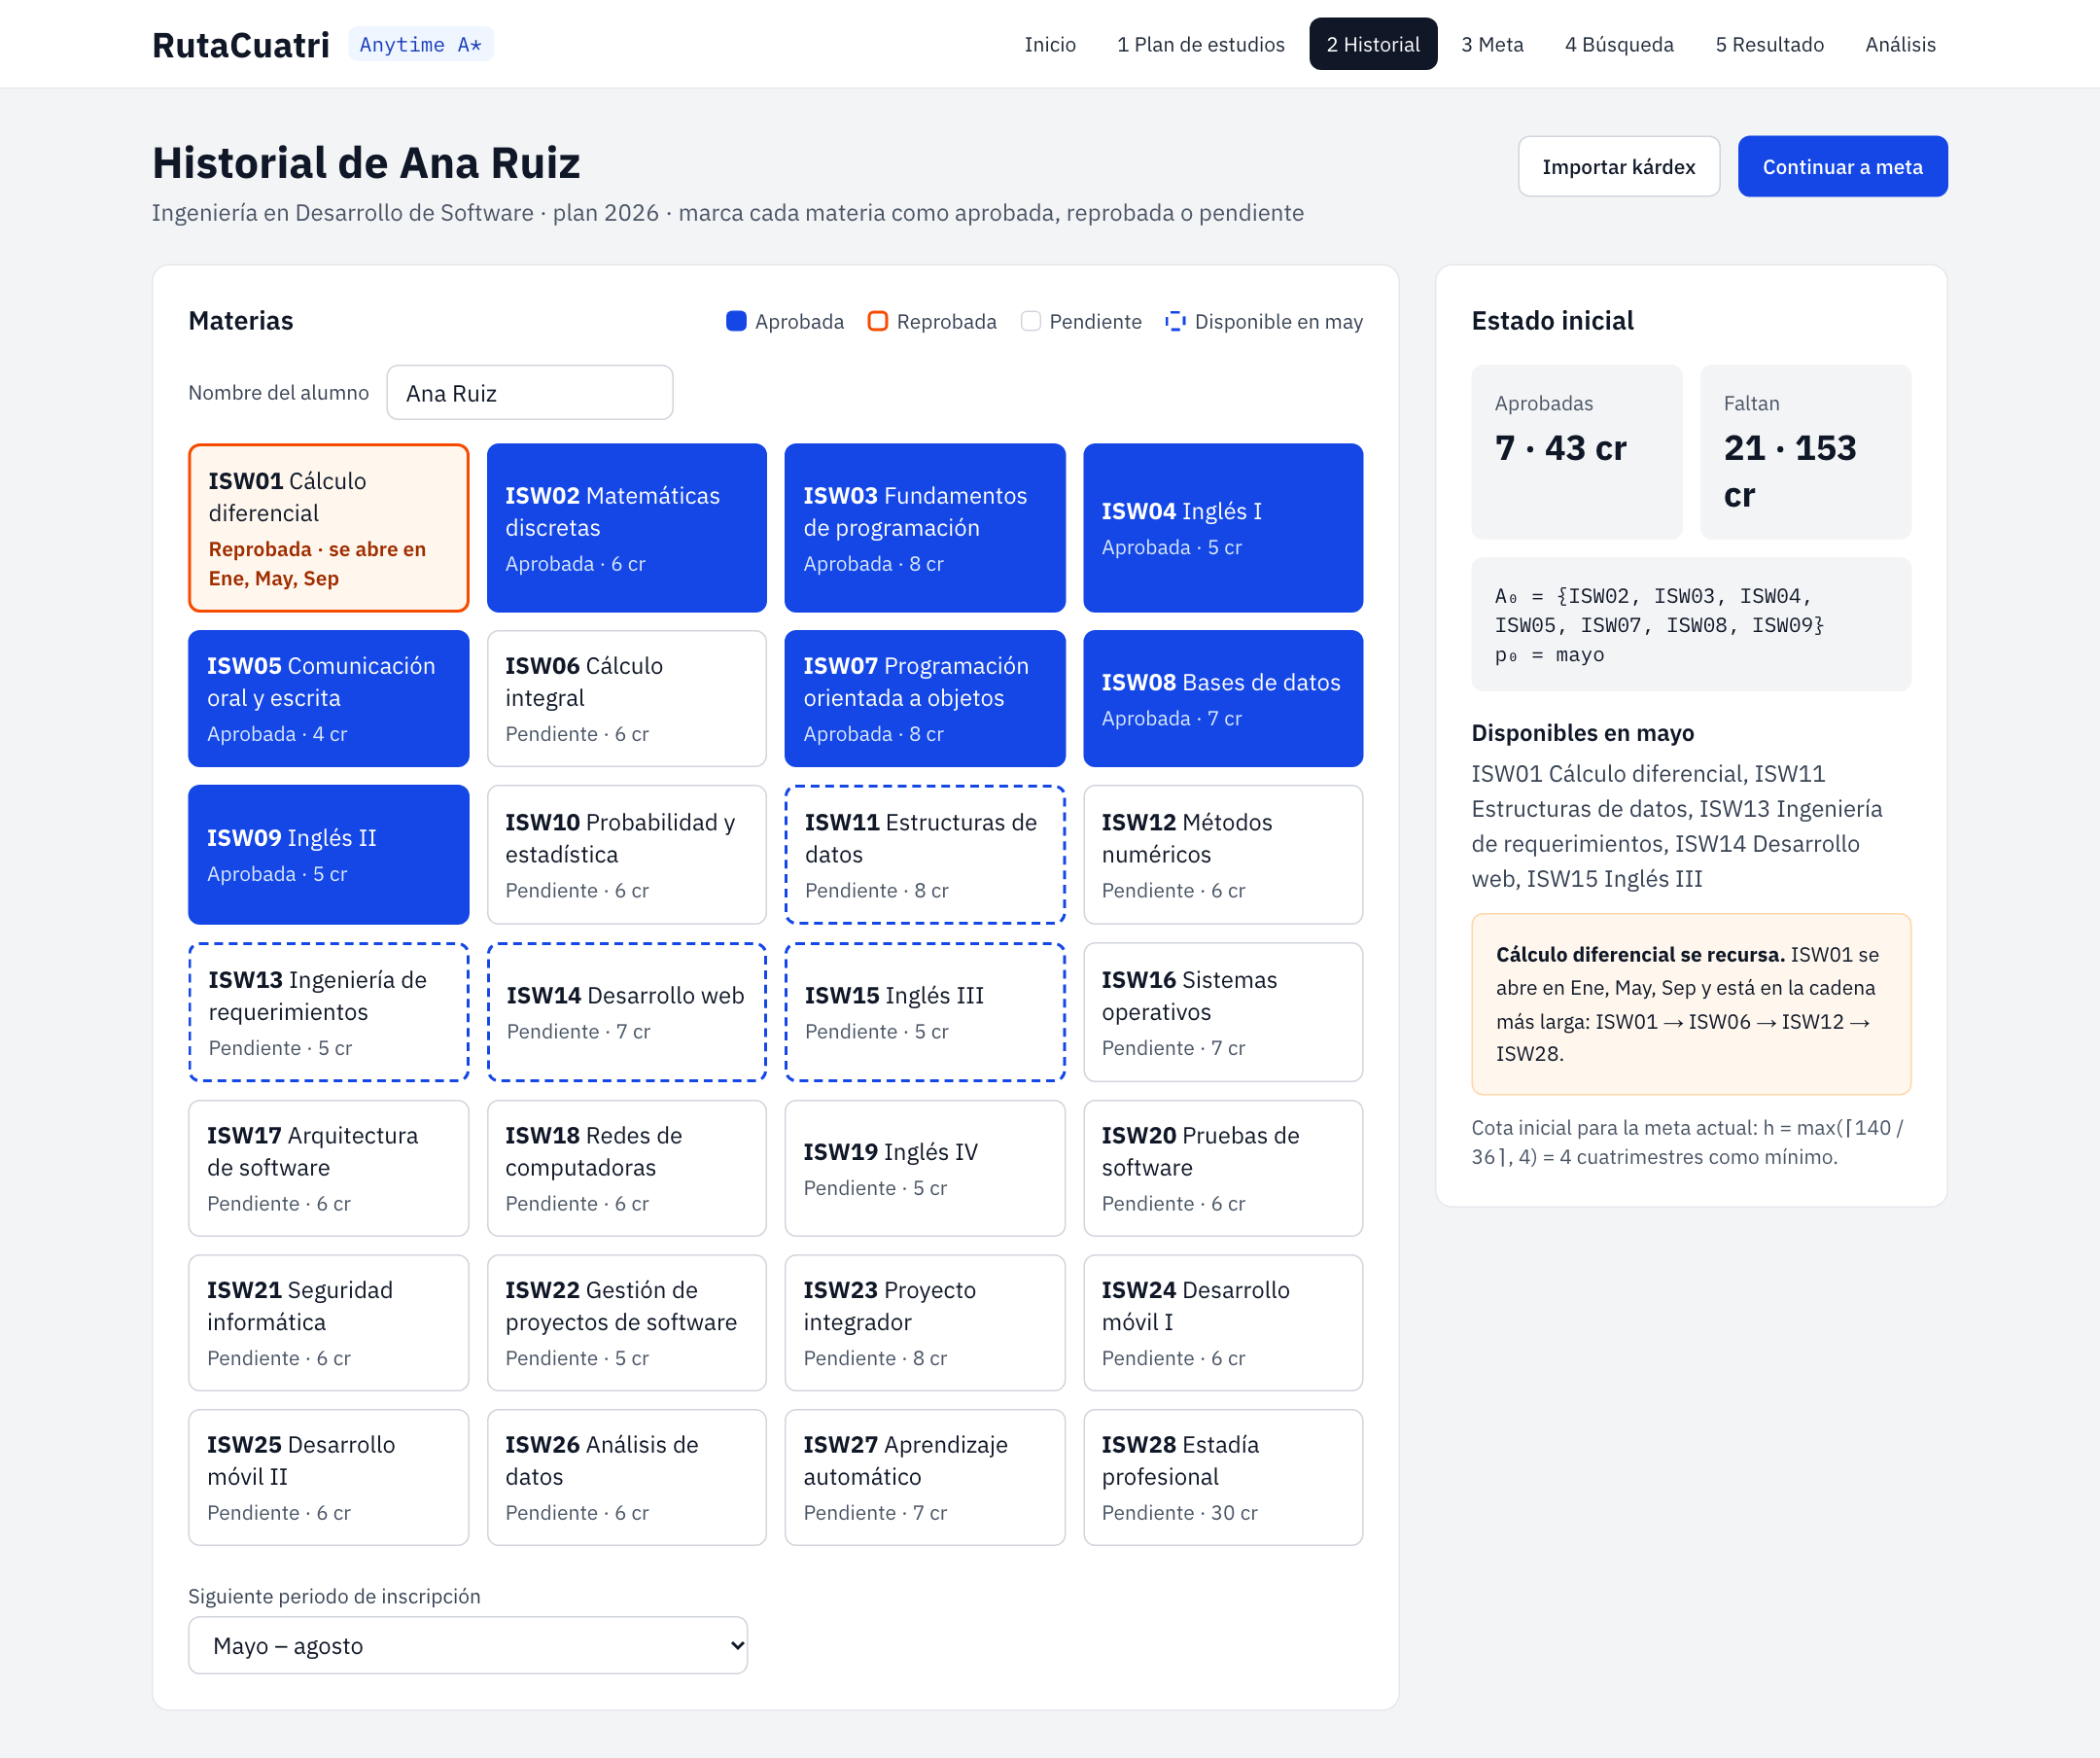
\includegraphics[width=\textwidth,height=0.75\textheight,keepaspectratio]{caso1-historial}
    \caption{Caso 1: historial de Ana Ruiz y estado inicial}
    \label{FIG::C1Historial}
\end{figure}

La meta es la titulación con especialidad A (M1) con el perfil regular ($C_{norm} = 30$, $C_{max} = 36$, $\beta = 0.1$, $K = 7$). La Figura~\ref{FIG::C1Meta} muestra la pantalla de meta y parámetros con el resumen del problema.

\begin{figure}[H]
    \centering
    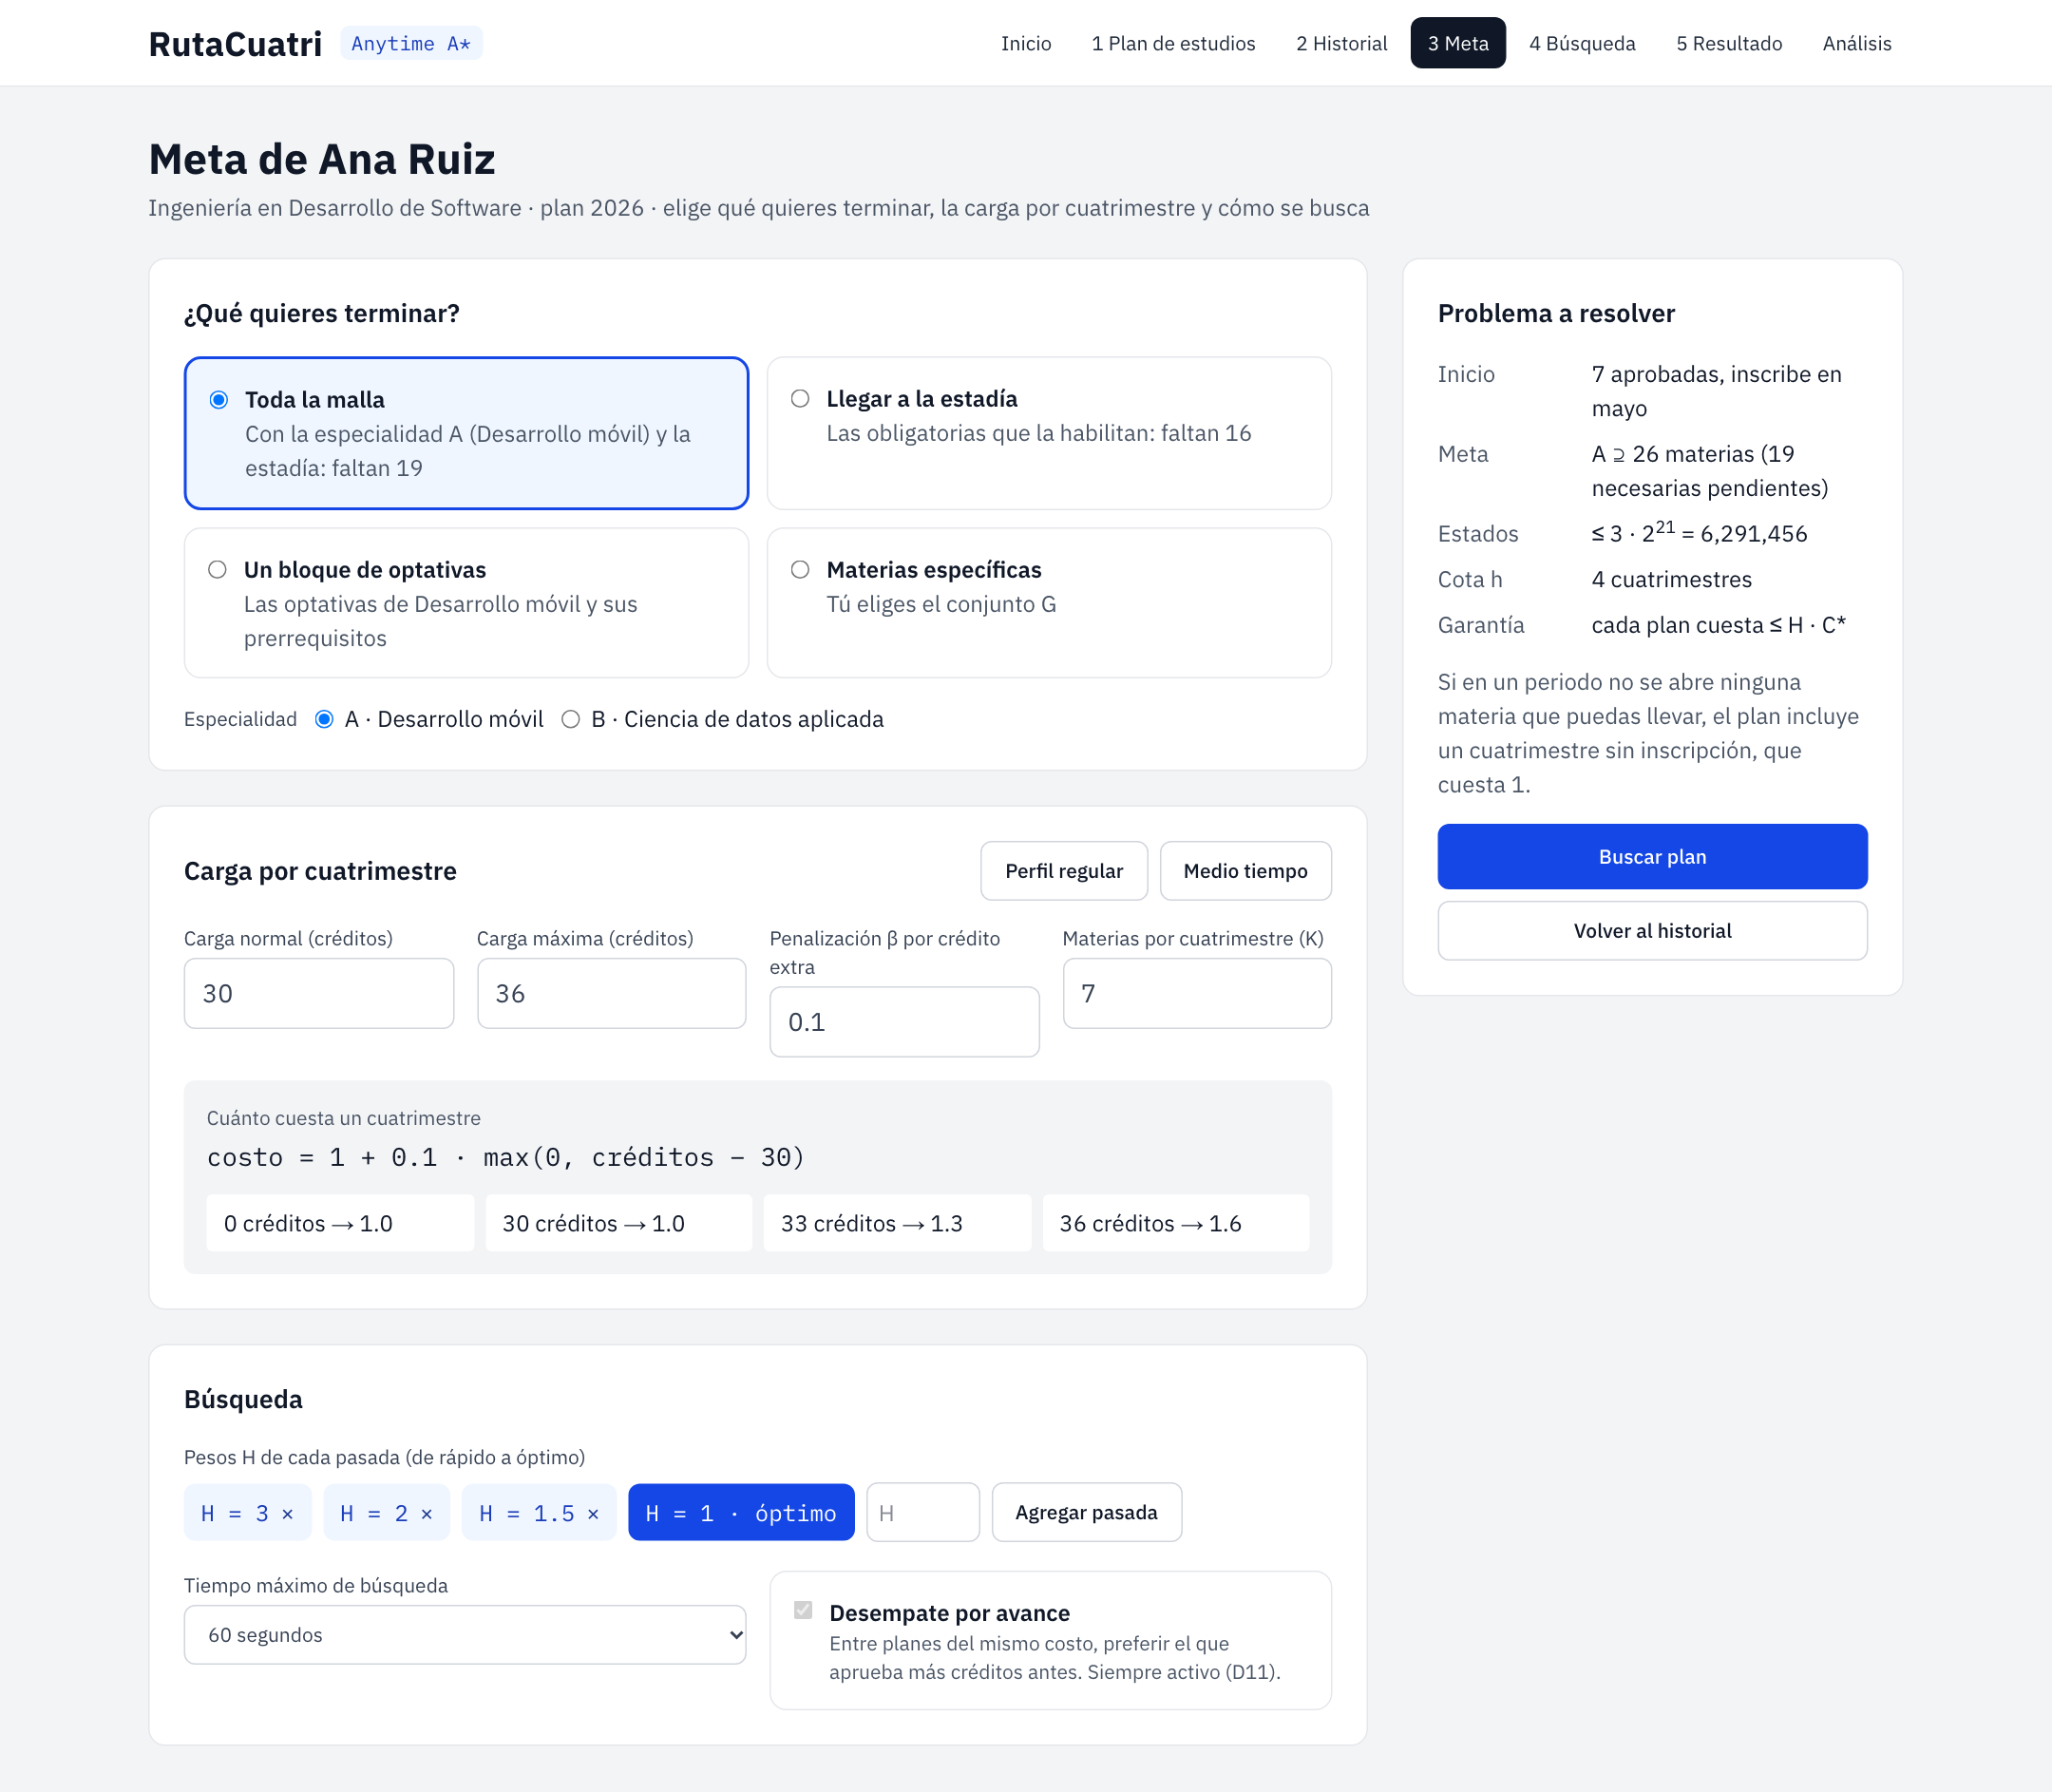
\includegraphics[width=\textwidth,height=0.75\textheight,keepaspectratio]{caso1-meta}
    \caption{Caso 1: meta y parámetros}
    \label{FIG::C1Meta}
\end{figure}

\subsection{Solución}
El plan óptimo tiene 5 cuatrimestres y costo 5.0, sin sobrecarga (Figura~\ref{FIG::C1Resultado}). Ana lleva Cálculo diferencial en su primer cuatrimestre, junto con Estructuras de datos, Ingeniería de requerimientos y Desarrollo web, y termina con la estadía en septiembre del segundo año. El panel derecho explica por qué son 5: la cota es 4 y la oferta obliga a un cuatrimestre más, porque Métodos numéricos (ISW12) solo se abre en mayo y septiembre.

\begin{figure}[H]
    \centering
    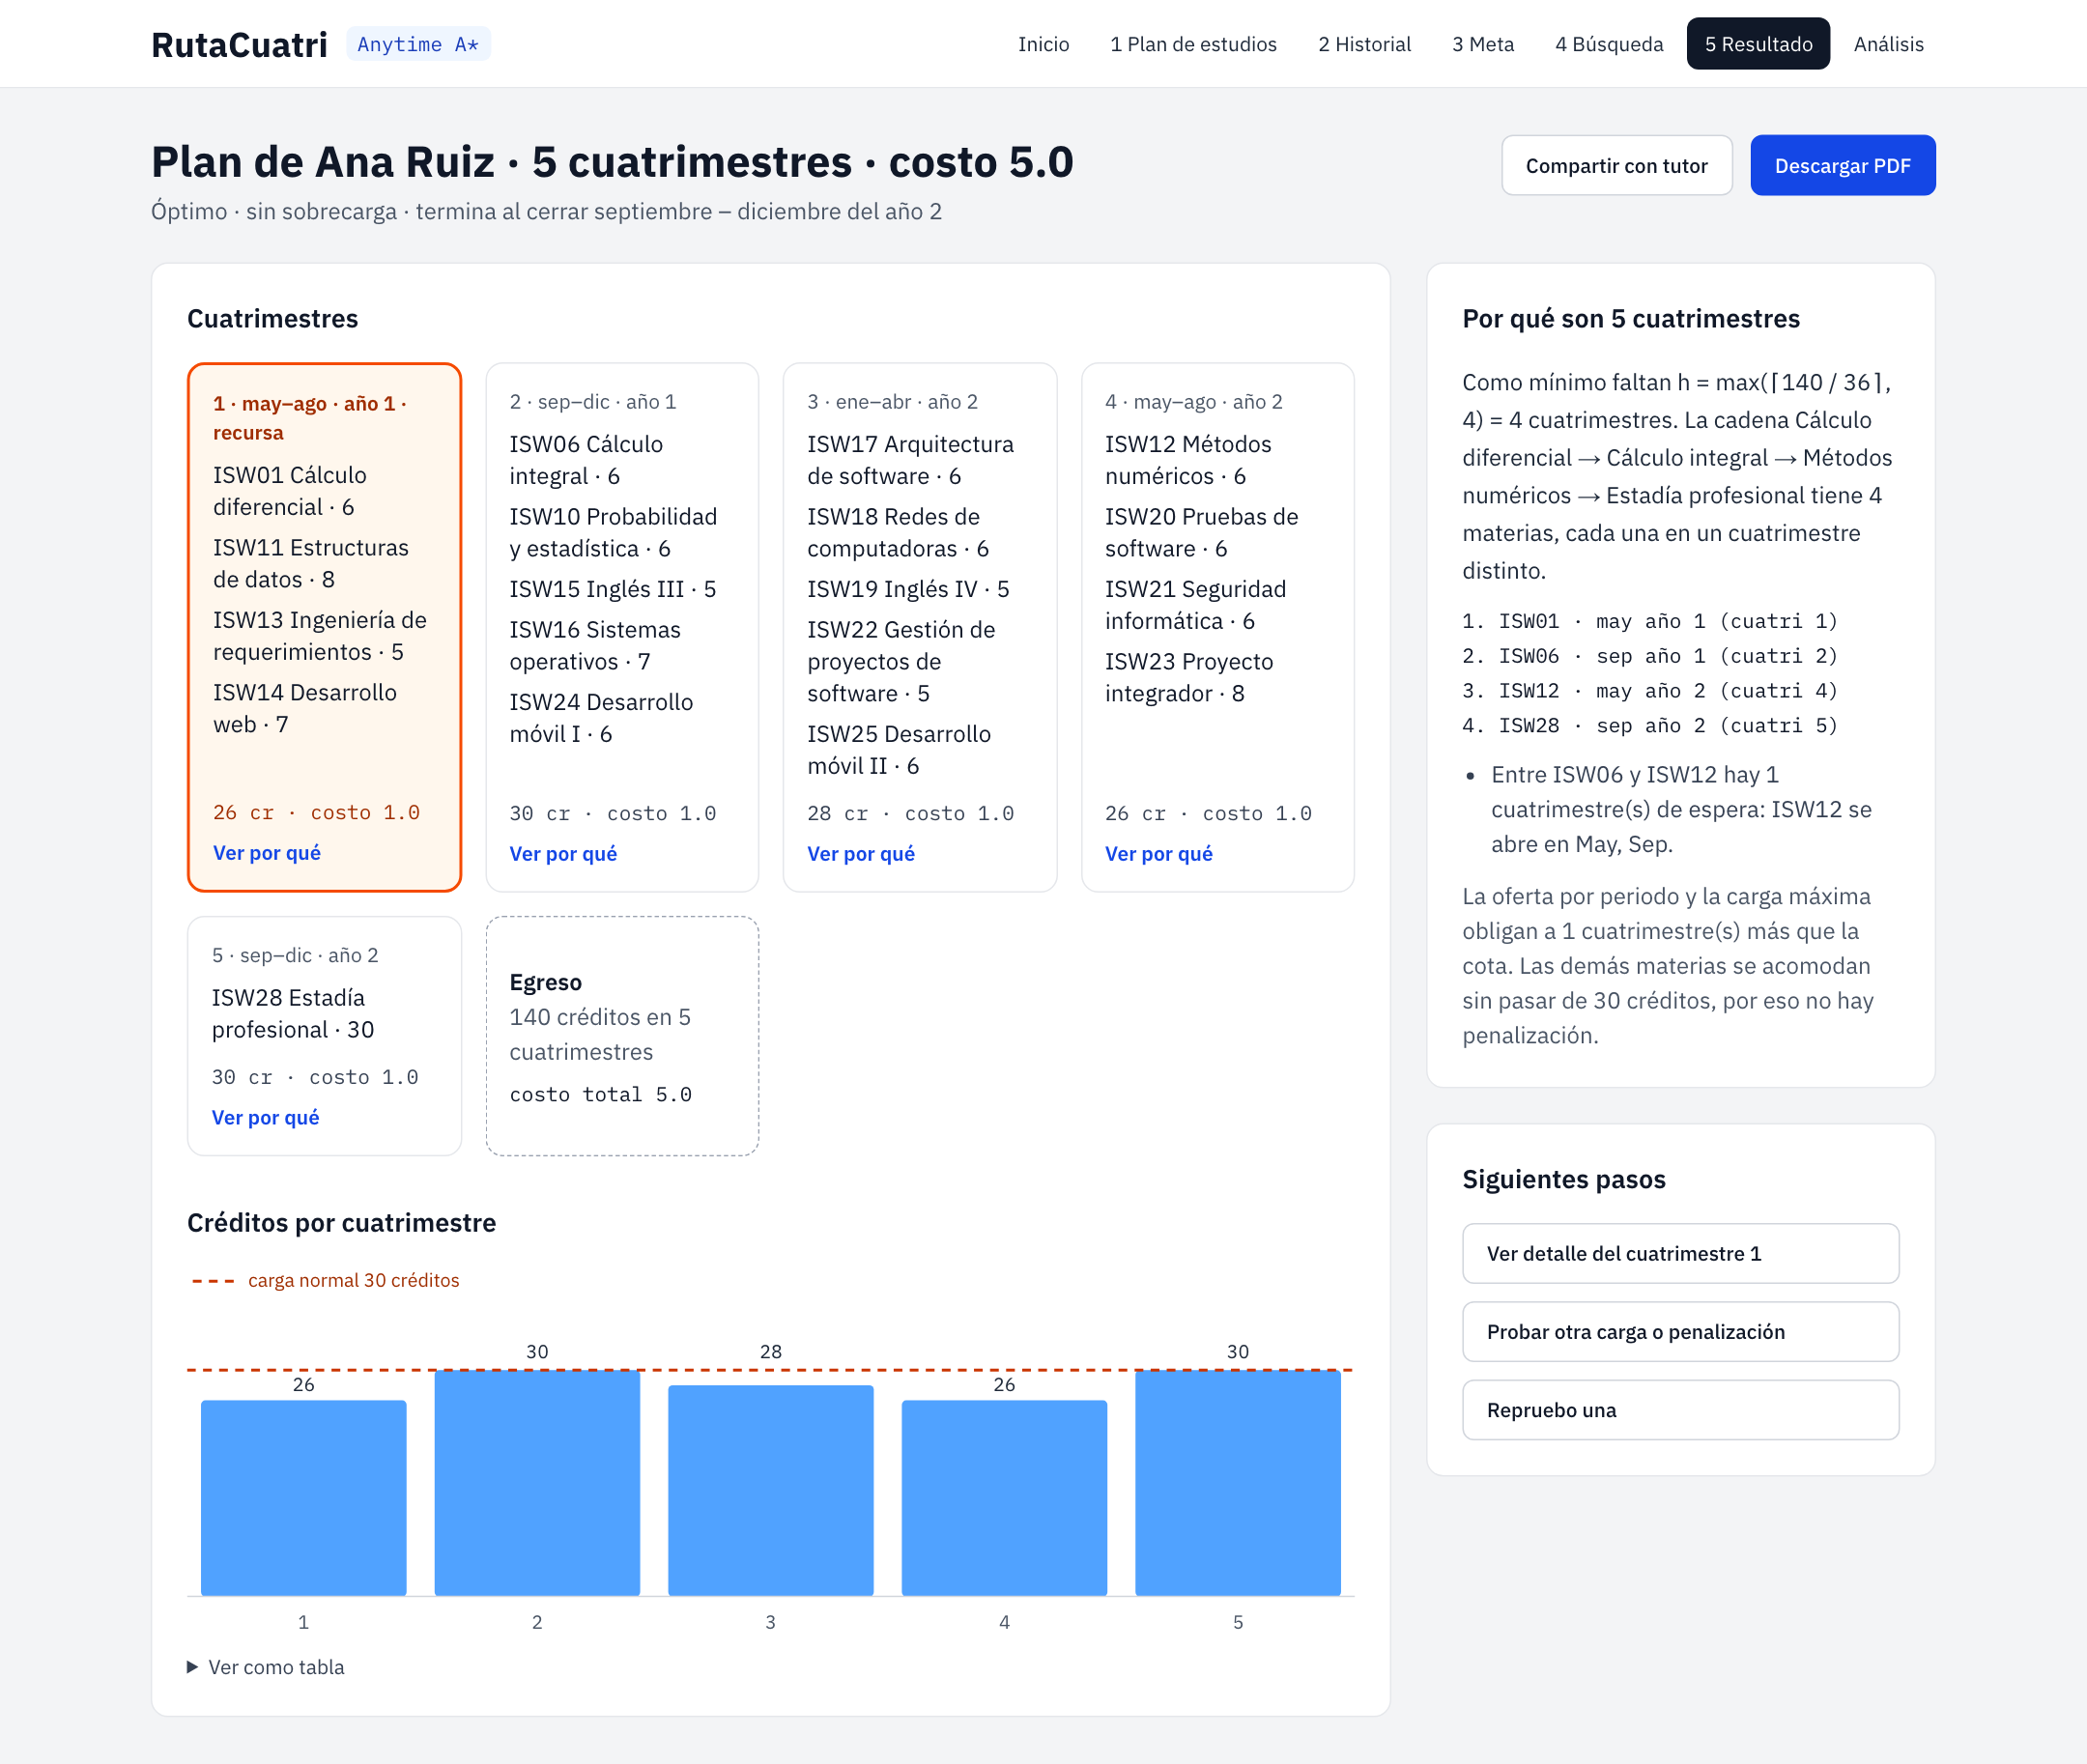
\includegraphics[width=\textwidth,height=0.75\textheight,keepaspectratio]{caso1-resultado}
    \caption{Caso 1: plan óptimo de Ana Ruiz}
    \label{FIG::C1Resultado}
\end{figure}

\subsection{Ejecución}
La búsqueda corre en el Worker y llena la tabla de pasadas (Figura~\ref{FIG::C1Busqueda}). La primera pasada ($H = 3$) encuentra un plan de 7.0 con 8 expansiones; la segunda ($H = 2$) lo mejora a 5.0 con 11; las pasadas con $H = 1.5$ y $H = 1$ expanden solo el estado inicial, porque todos sus sucesores tienen $g + h \geq 5.0$. Eso prueba que 5.0 es el óptimo.

\begin{figure}[H]
    \centering
    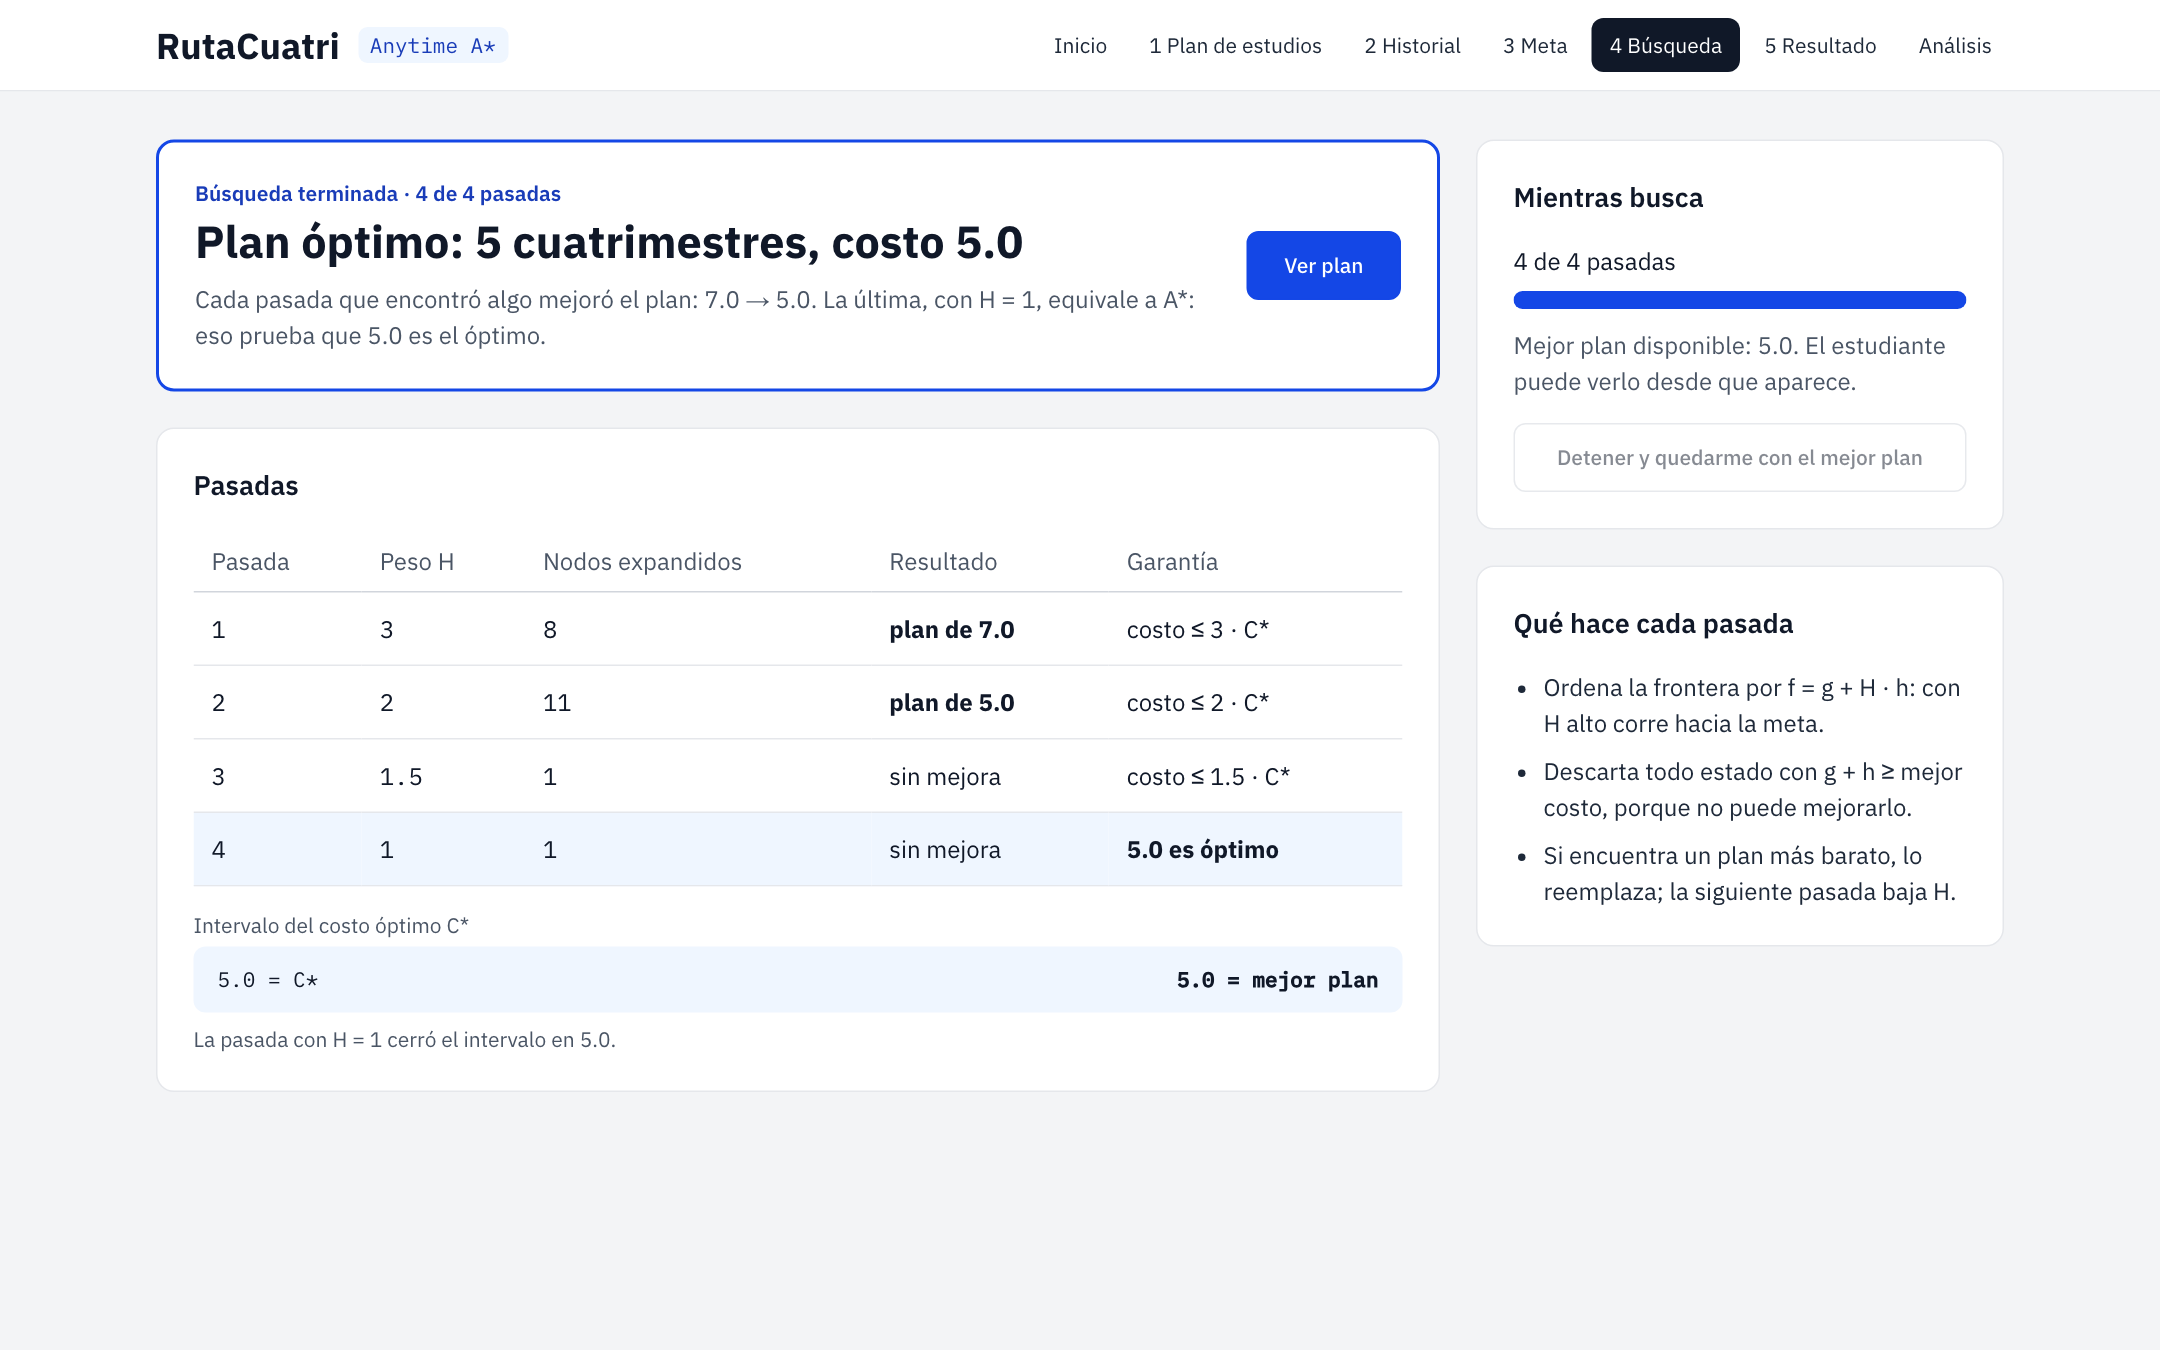
\includegraphics[width=\textwidth,height=0.75\textheight,keepaspectratio]{caso1-busqueda}
    \caption{Caso 1: pasadas de Anytime A*}
    \label{FIG::C1Busqueda}
\end{figure}

La Figura~\ref{FIG::C1Detalle} muestra el detalle del primer cuatrimestre: las materias inscritas y la pospuesta, y las alternativas con su costo total calculado con A* desde el estado que deja cada una (son los sucesores de la Tabla~\ref{TAB::TransicionesAna}). La elegida tiene el menor costo total y el estado $n'$ que deja cumple $f(n') = 1.0 + 4 = 5.0 \leq 5.0$.

\begin{figure}[H]
    \centering
    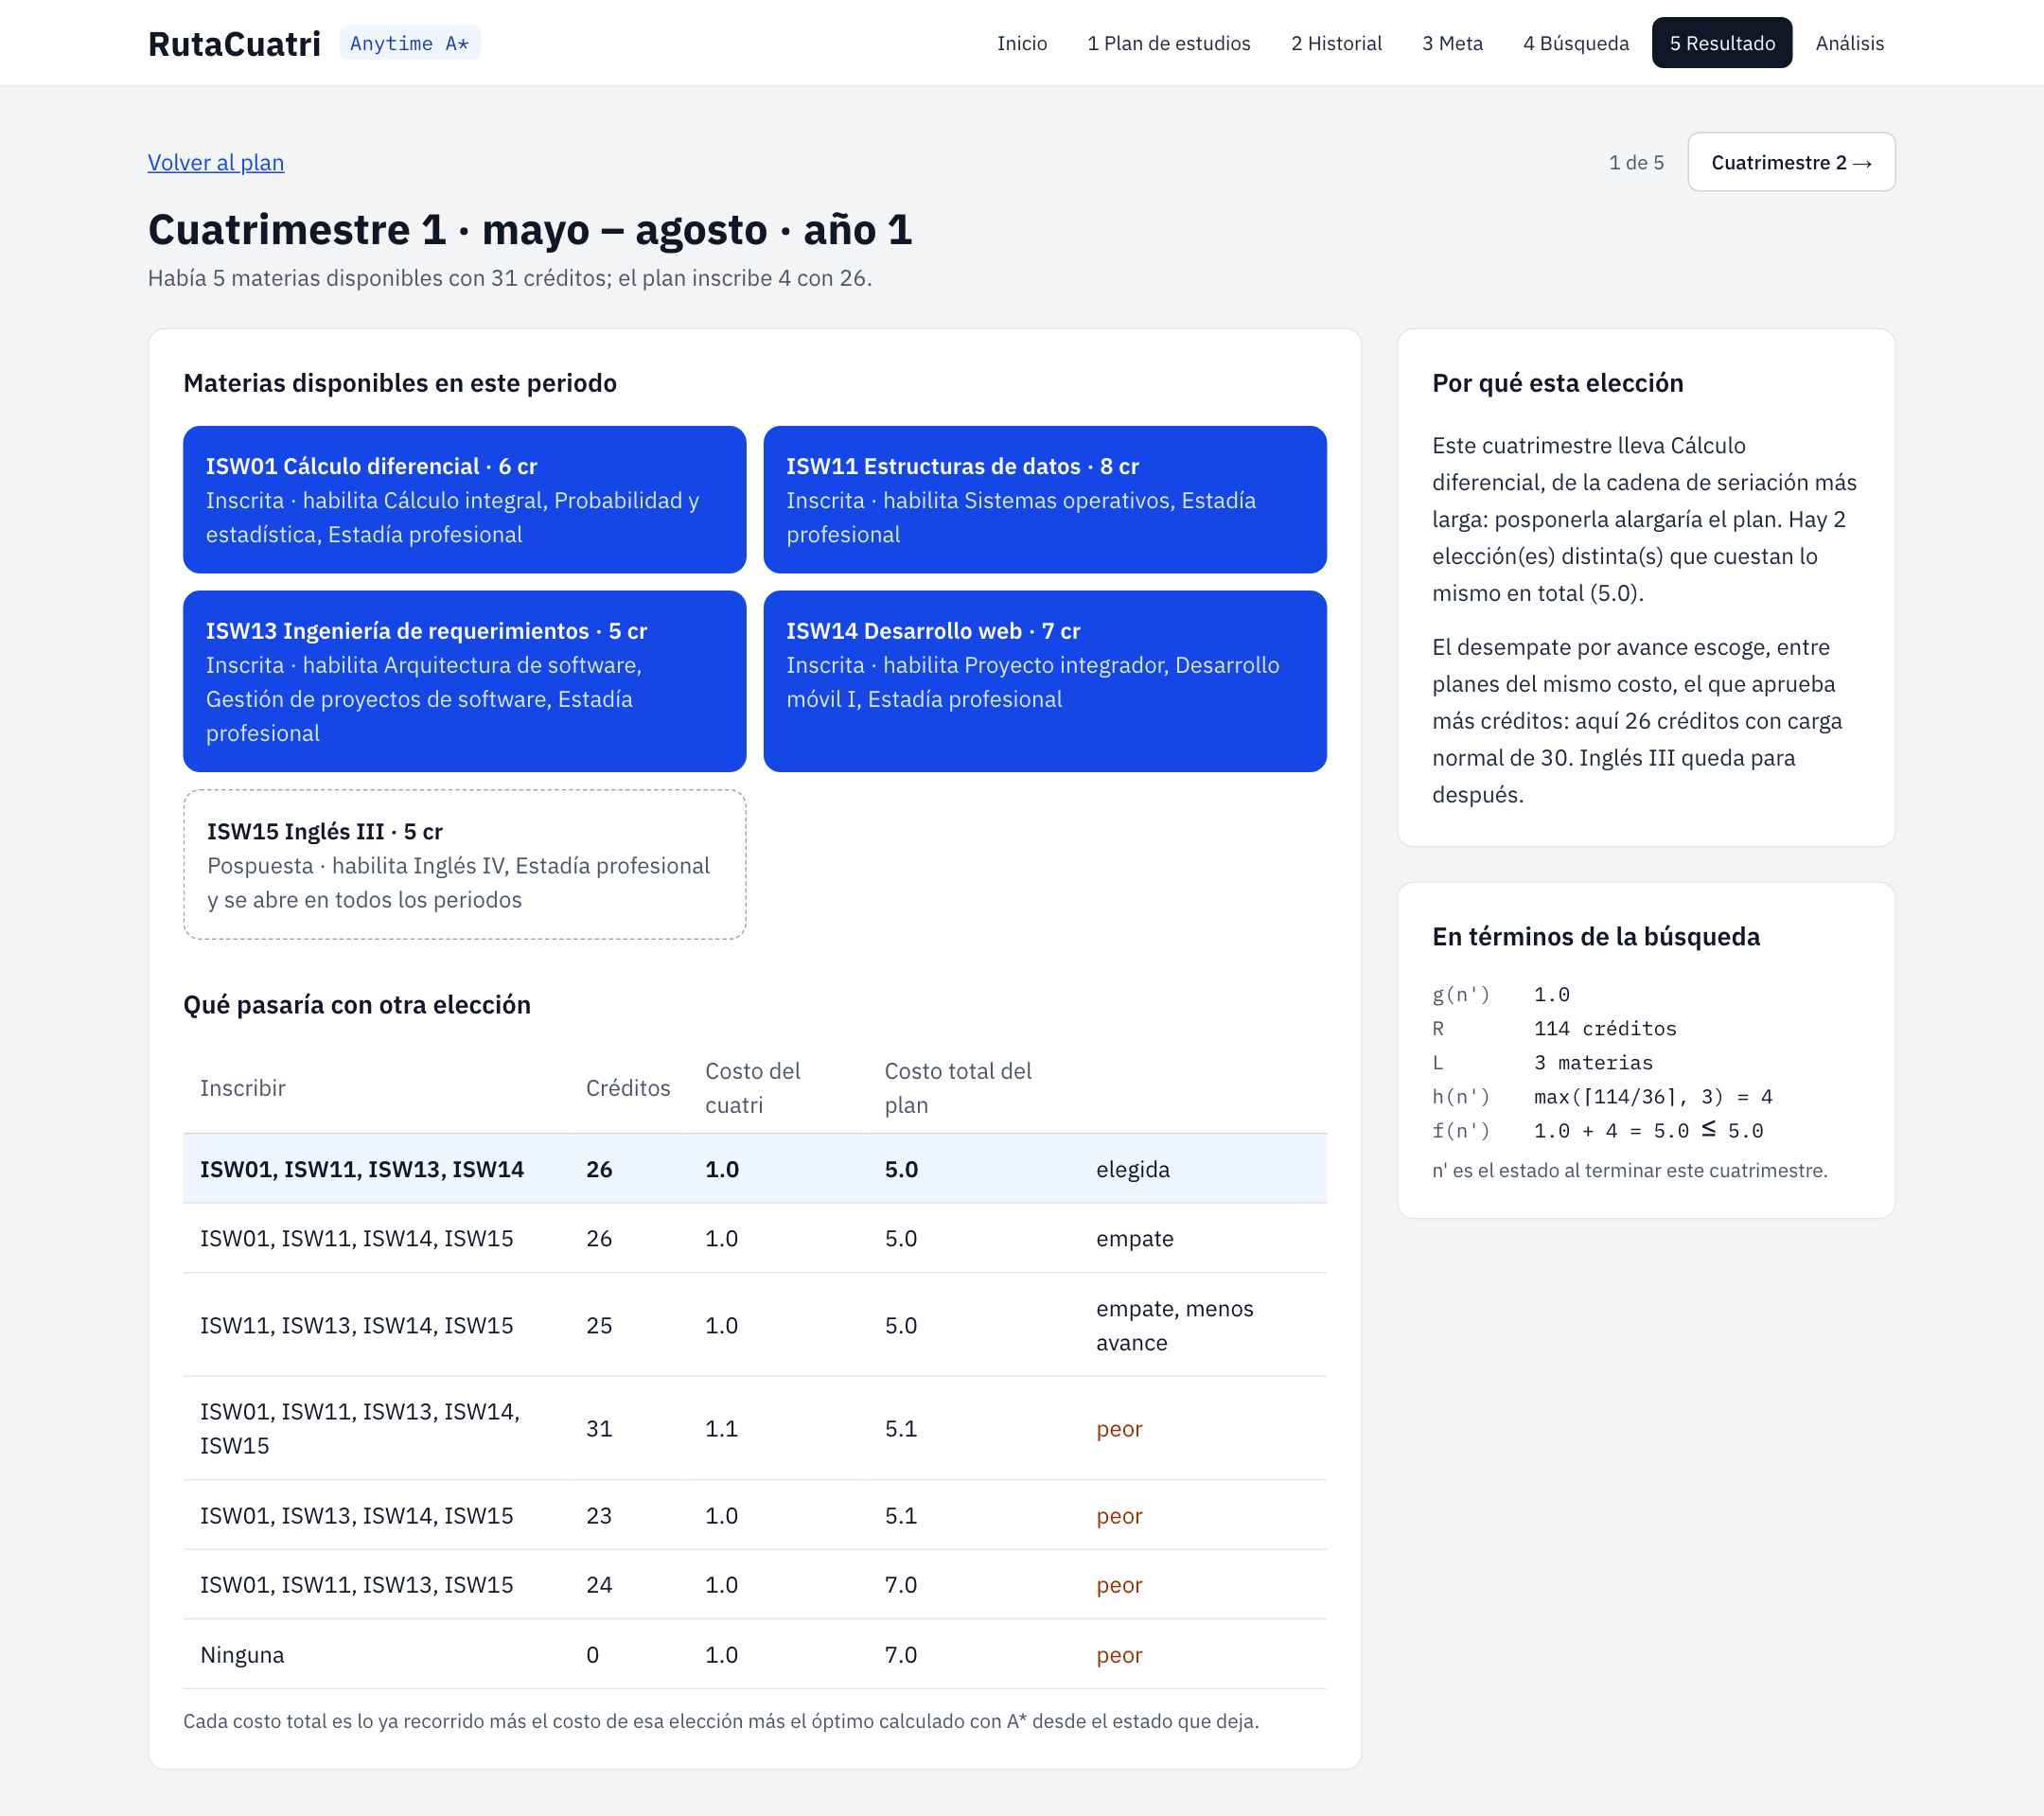
\includegraphics[width=\textwidth,height=0.8\textheight,keepaspectratio]{caso1-detalle}
    \caption{Caso 1: detalle del primer cuatrimestre y sus alternativas}
    \label{FIG::C1Detalle}
\end{figure}

Por último, la Figura~\ref{FIG::C1Celular} muestra la vista de celular con la opción ``Repruebo una''. Si Ana vuelve a reprobar Cálculo diferencial en su primer cuatrimestre, el sistema marca las otras tres materias como aprobadas, deja Cálculo diferencial como reprobada y vuelve a buscar desde septiembre: le quedan 4 cuatrimestres con costo 4.0.

\begin{figure}[H]
    \centering
    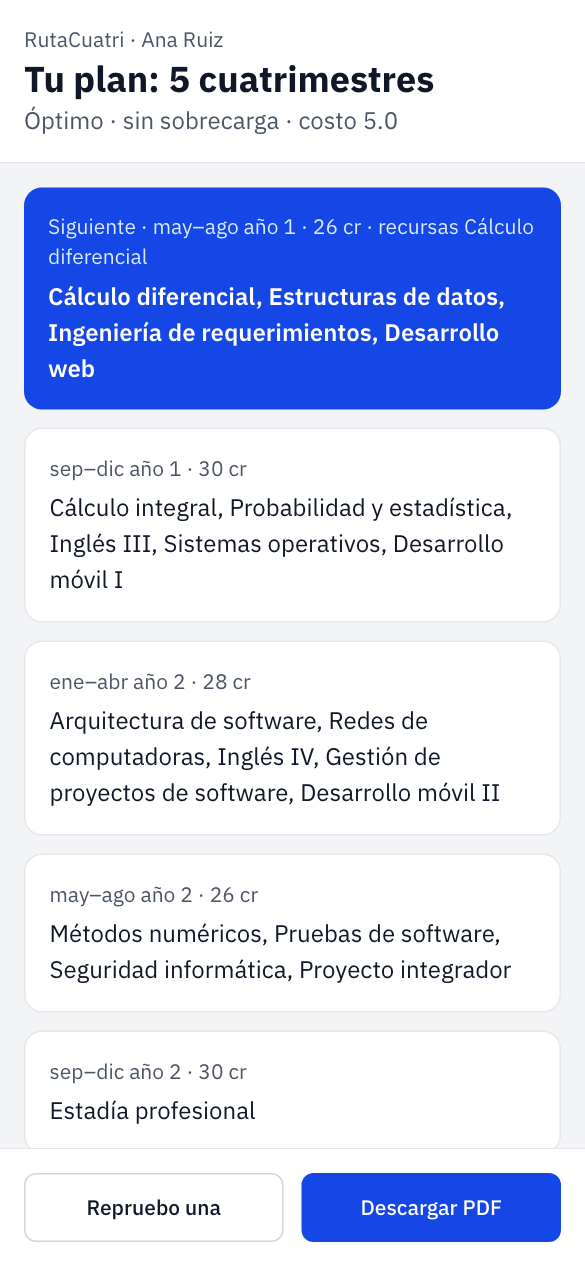
\includegraphics[width=0.31\textwidth]{caso1-celular}\hfill
    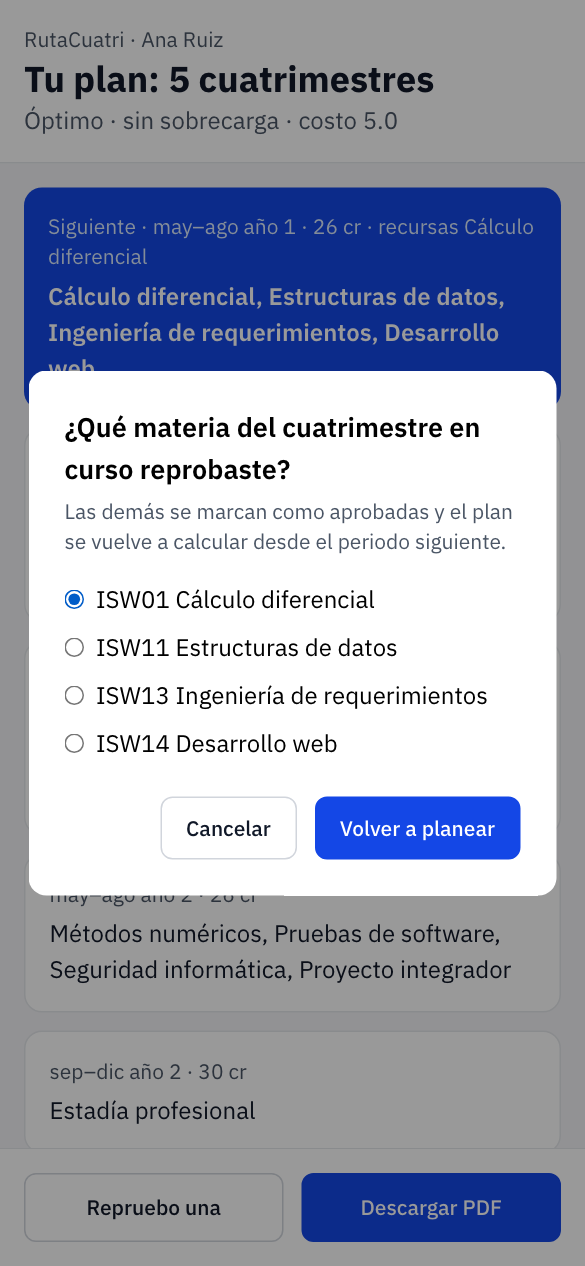
\includegraphics[width=0.31\textwidth]{caso1-repruebo}\hfill
    
\includegraphics[width=0.31\textwidth]{caso1-replaneado}
    \caption{Caso 1: vista de celular, ``Repruebo una'' y plan recalculado}
    \label{FIG::C1Celular}
\end{figure}

\subsection{Comentarios}
Con la carga regular, Ana termina en septiembre del segundo año, en 5 cuatrimestres: uno más que la cota, por la espera de Métodos numéricos. La cadena ISW01 $\to$ ISW06 $\to$ ISW12 $\to$ ISW28 marca el ritmo, y por eso el plan inscribe Cálculo diferencial en el primer cuatrimestre. Incluso si lo reprueba otra vez, el plan recalculado sigue terminando en el mismo septiembre. La primera pasada dio un plan 40\% más caro que el óptimo (7.0 contra 5.0), lejos de su garantía de $3 \cdot C^*$, y la segunda ya llegó al óptimo.

\section{Caso 2: nuevo ingreso con carga de medio tiempo}

\subsection{Descripción}
Un estudiante de nuevo ingreso de ISW trabaja y solo puede llevar carga de medio tiempo. Quiere terminar toda la carrera con la especialidad A. Es el escenario más difícil de los 72: las 26 materias son necesarias y, con $C_{norm} = 24$, el estudiante ya no cabe en un nivel por cuatrimestre, así que la búsqueda tiene que negociar entre cargar de más y alargar la carrera.

\subsection{Estado inicial y meta}
El estado inicial es $(\emptyset, \text{Sep})$ y la meta es M1. En la pantalla de meta se eligió el perfil de medio tiempo ($C_{norm} = 24$, $C_{max} = 30$); el resumen muestra hasta $3 \cdot 2^{28} = 805{,}306{,}368$ estados y una cota inicial de 7 cuatrimestres (Figura~\ref{FIG::C2Meta}).

\begin{figure}[H]
    \centering
    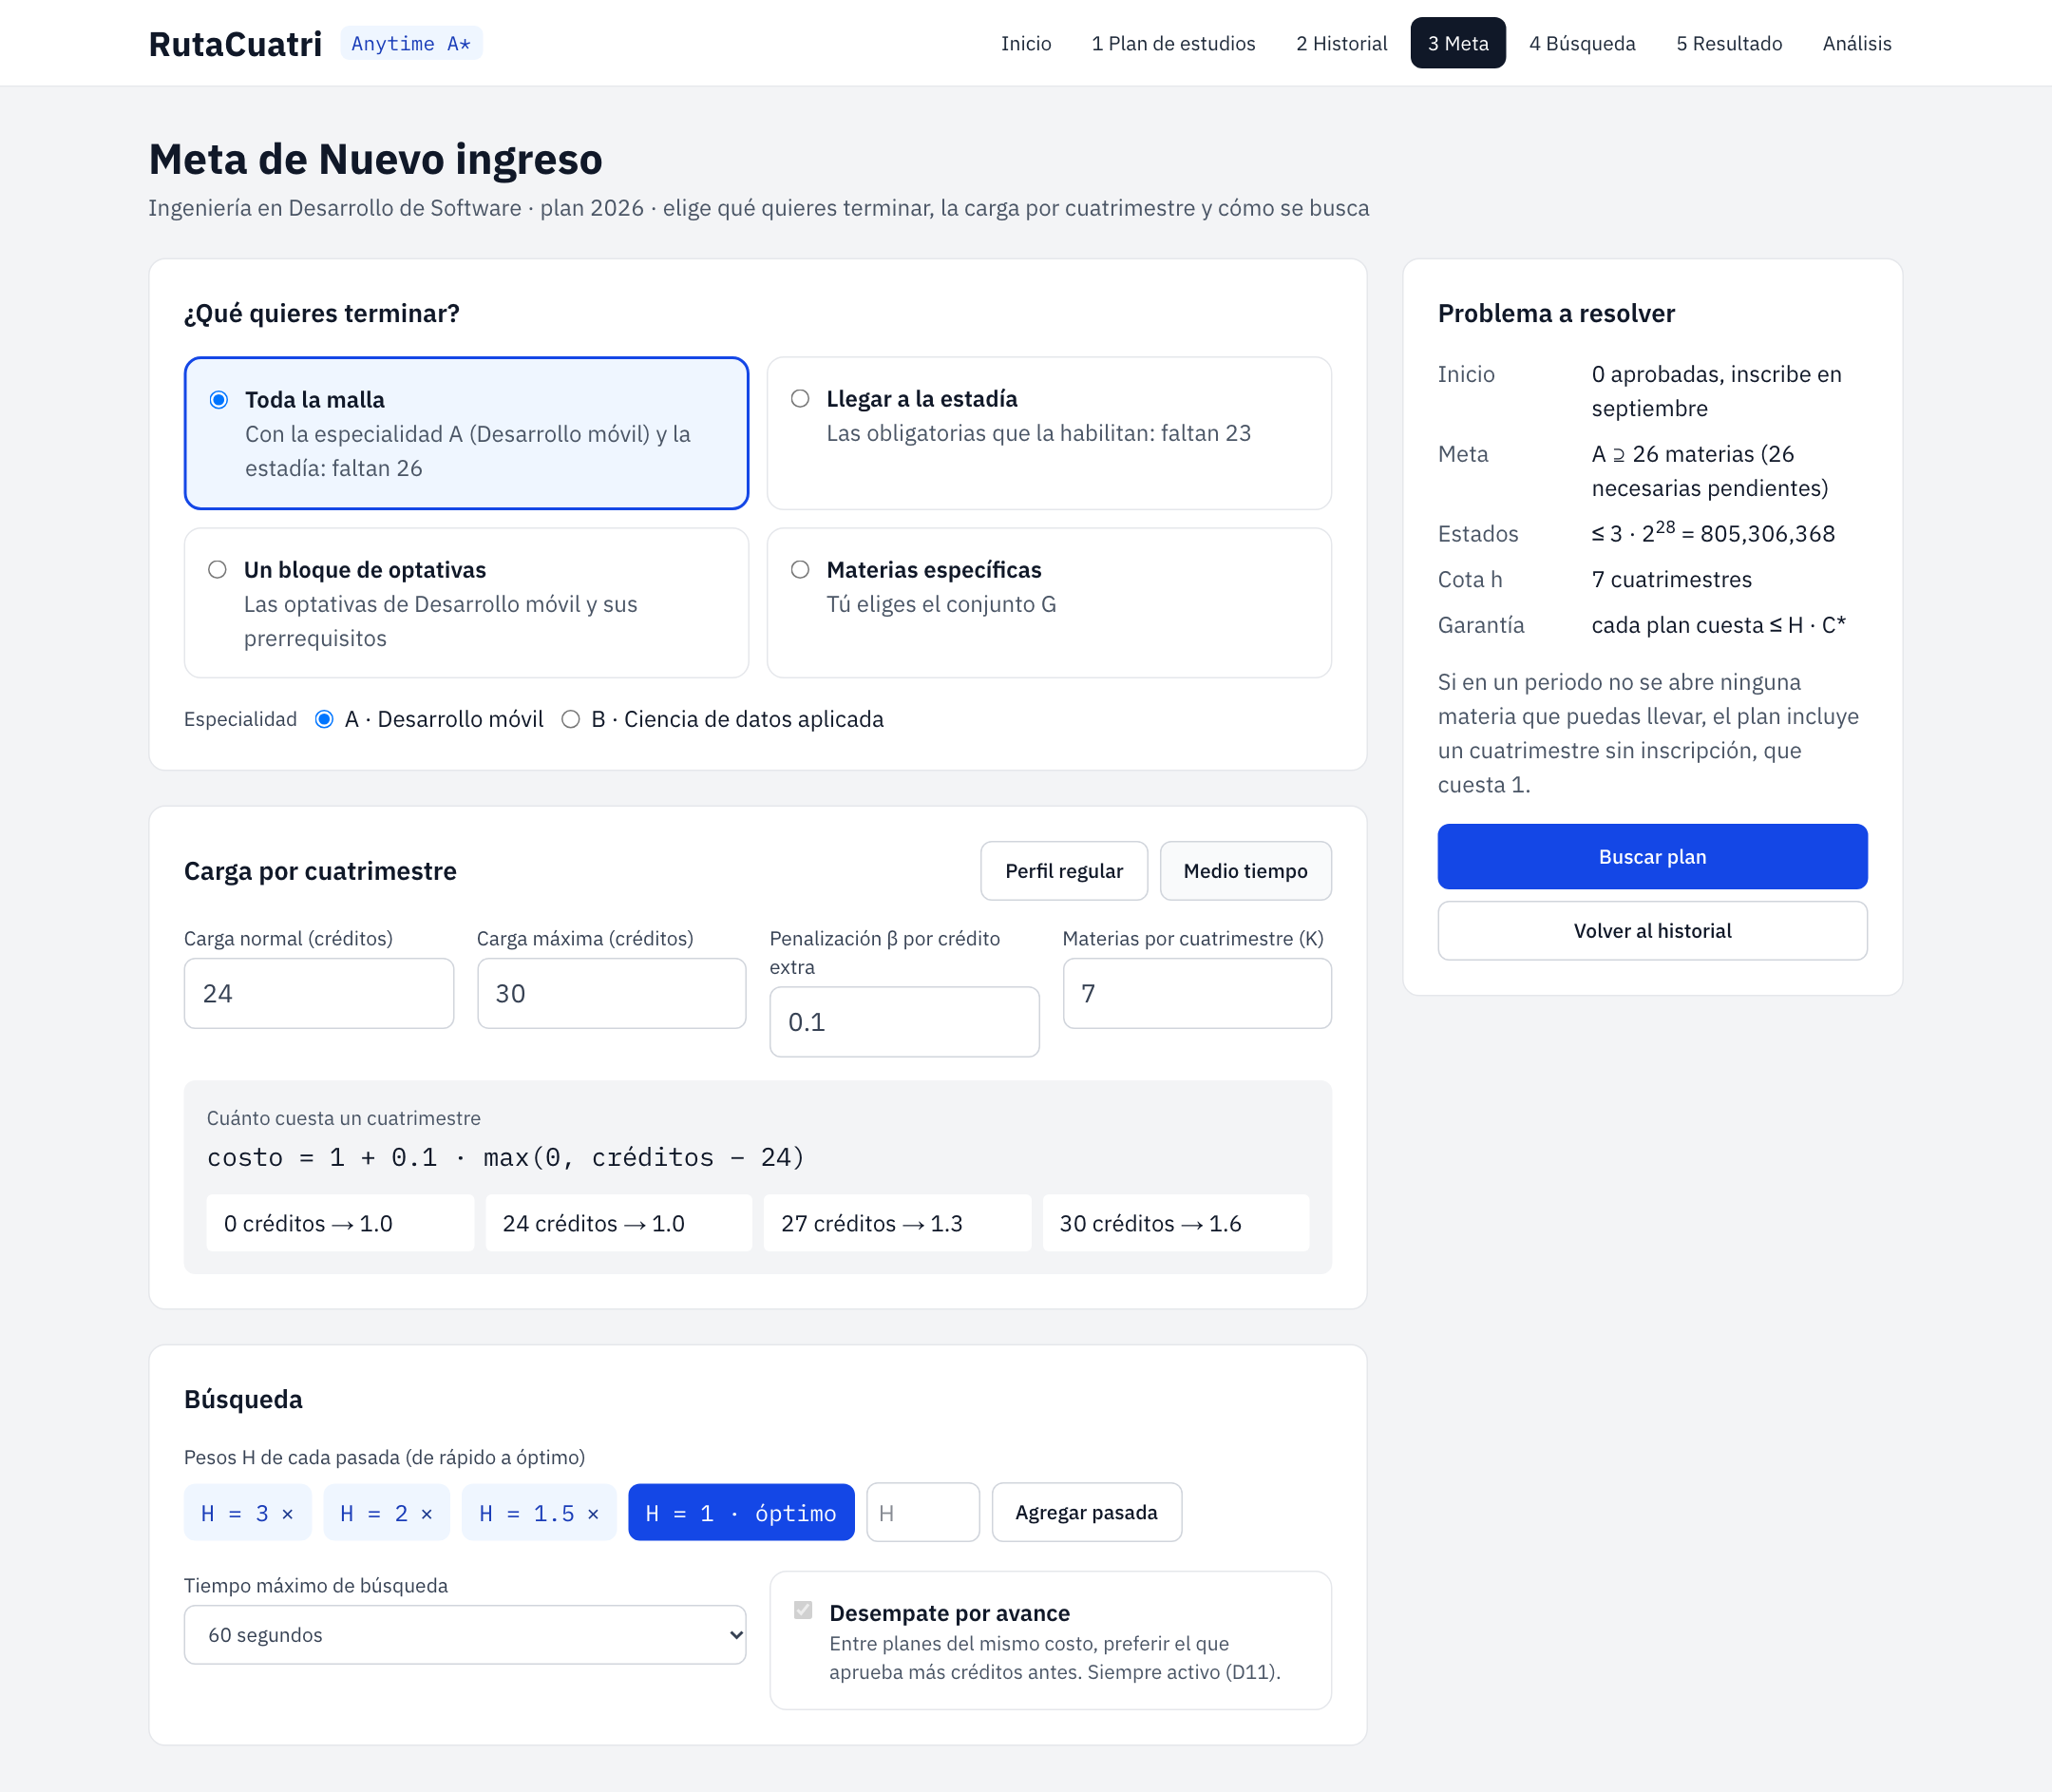
\includegraphics[width=\textwidth,height=0.75\textheight,keepaspectratio]{caso2-meta}
    \caption{Caso 2: meta y perfil de medio tiempo}
    \label{FIG::C2Meta}
\end{figure}

\subsection{Solución}
El plan óptimo tiene 7 cuatrimestres y costo 8.5 (Figura~\ref{FIG::C2Resultado}). Lleva 15 créditos de sobrecarga repartidos en cuatro cuatrimestres; la gráfica de créditos los marca en naranja sobre la línea de la carga normal.

\begin{figure}[H]
    \centering
    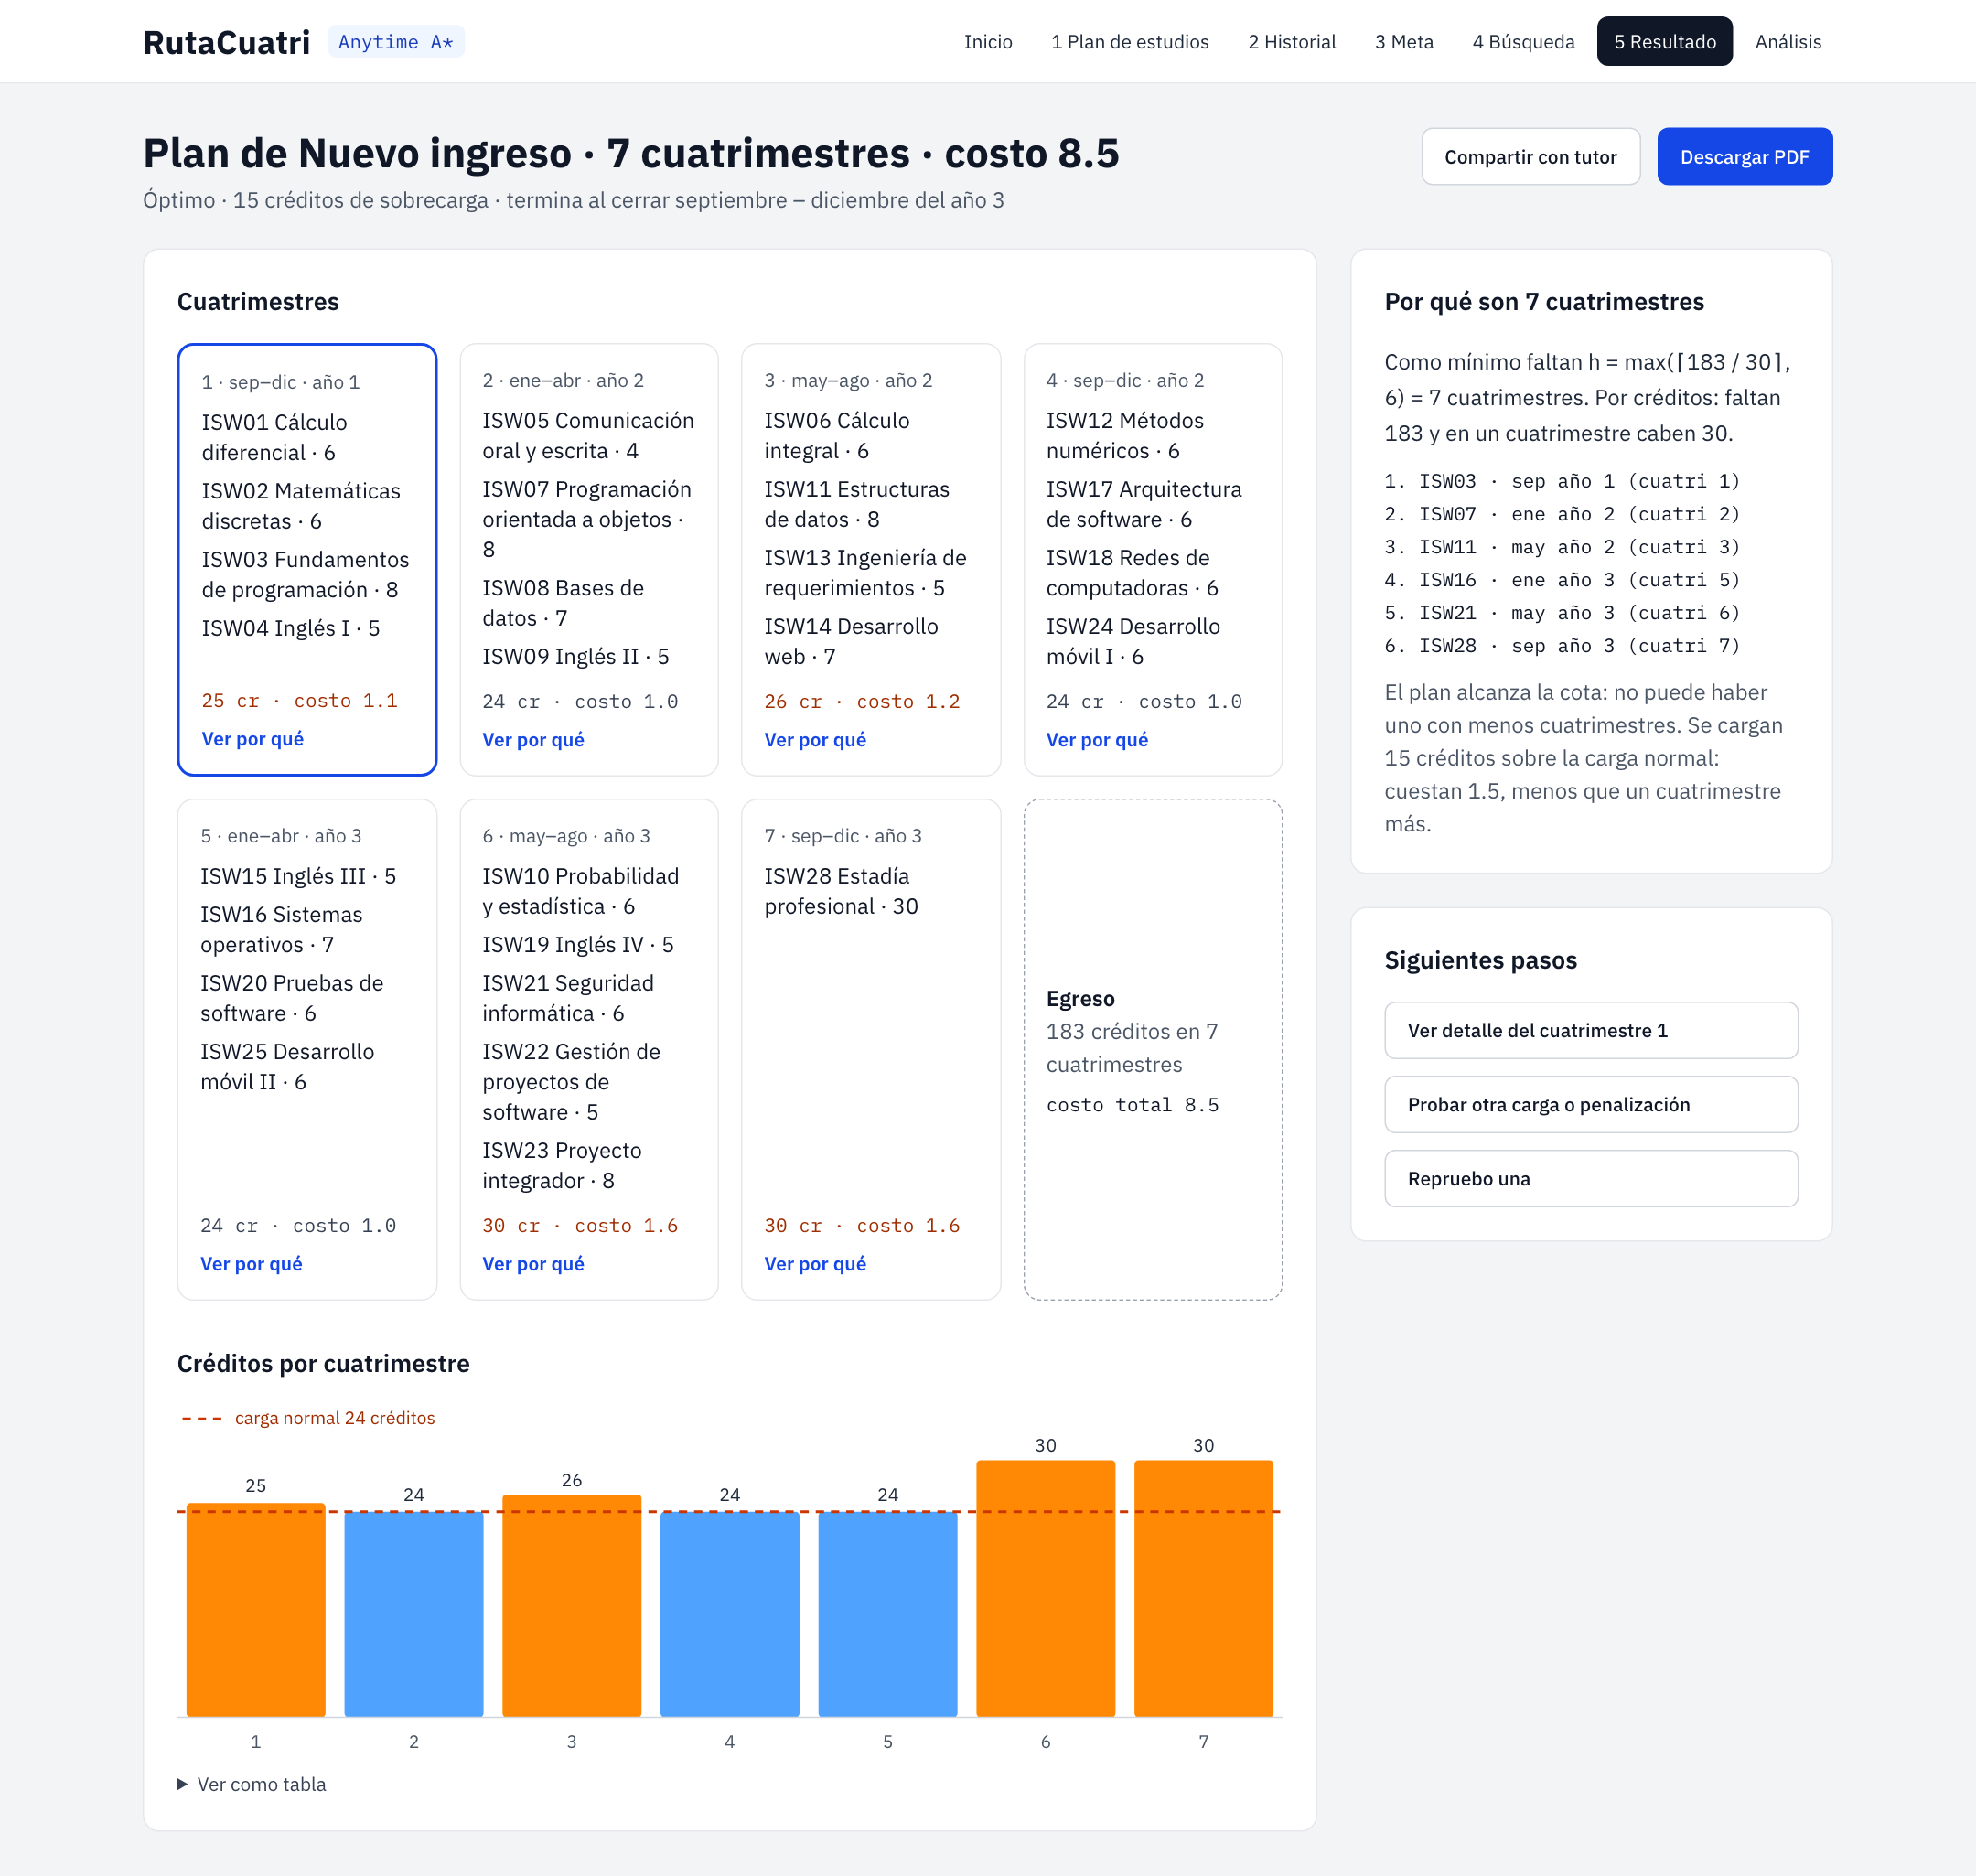
\includegraphics[width=\textwidth,height=0.75\textheight,keepaspectratio]{caso2-resultado}
    \caption{Caso 2: plan óptimo con carga de medio tiempo}
    \label{FIG::C2Resultado}
\end{figure}

\subsection{Ejecución}
Aquí las cuatro pasadas mejoran el plan (Figura~\ref{FIG::C2Busqueda}): 10.0 con 17 expansiones, 9.6 con 22, 8.8 con 77 y 8.5 con 2,918. El primer plan sale en 0.2 ms y el óptimo queda demostrado en 38 ms. Desde la primera pasada el estudiante sabe que el óptimo está entre $h = 7$ y 10.0.

\begin{figure}[H]
    \centering
    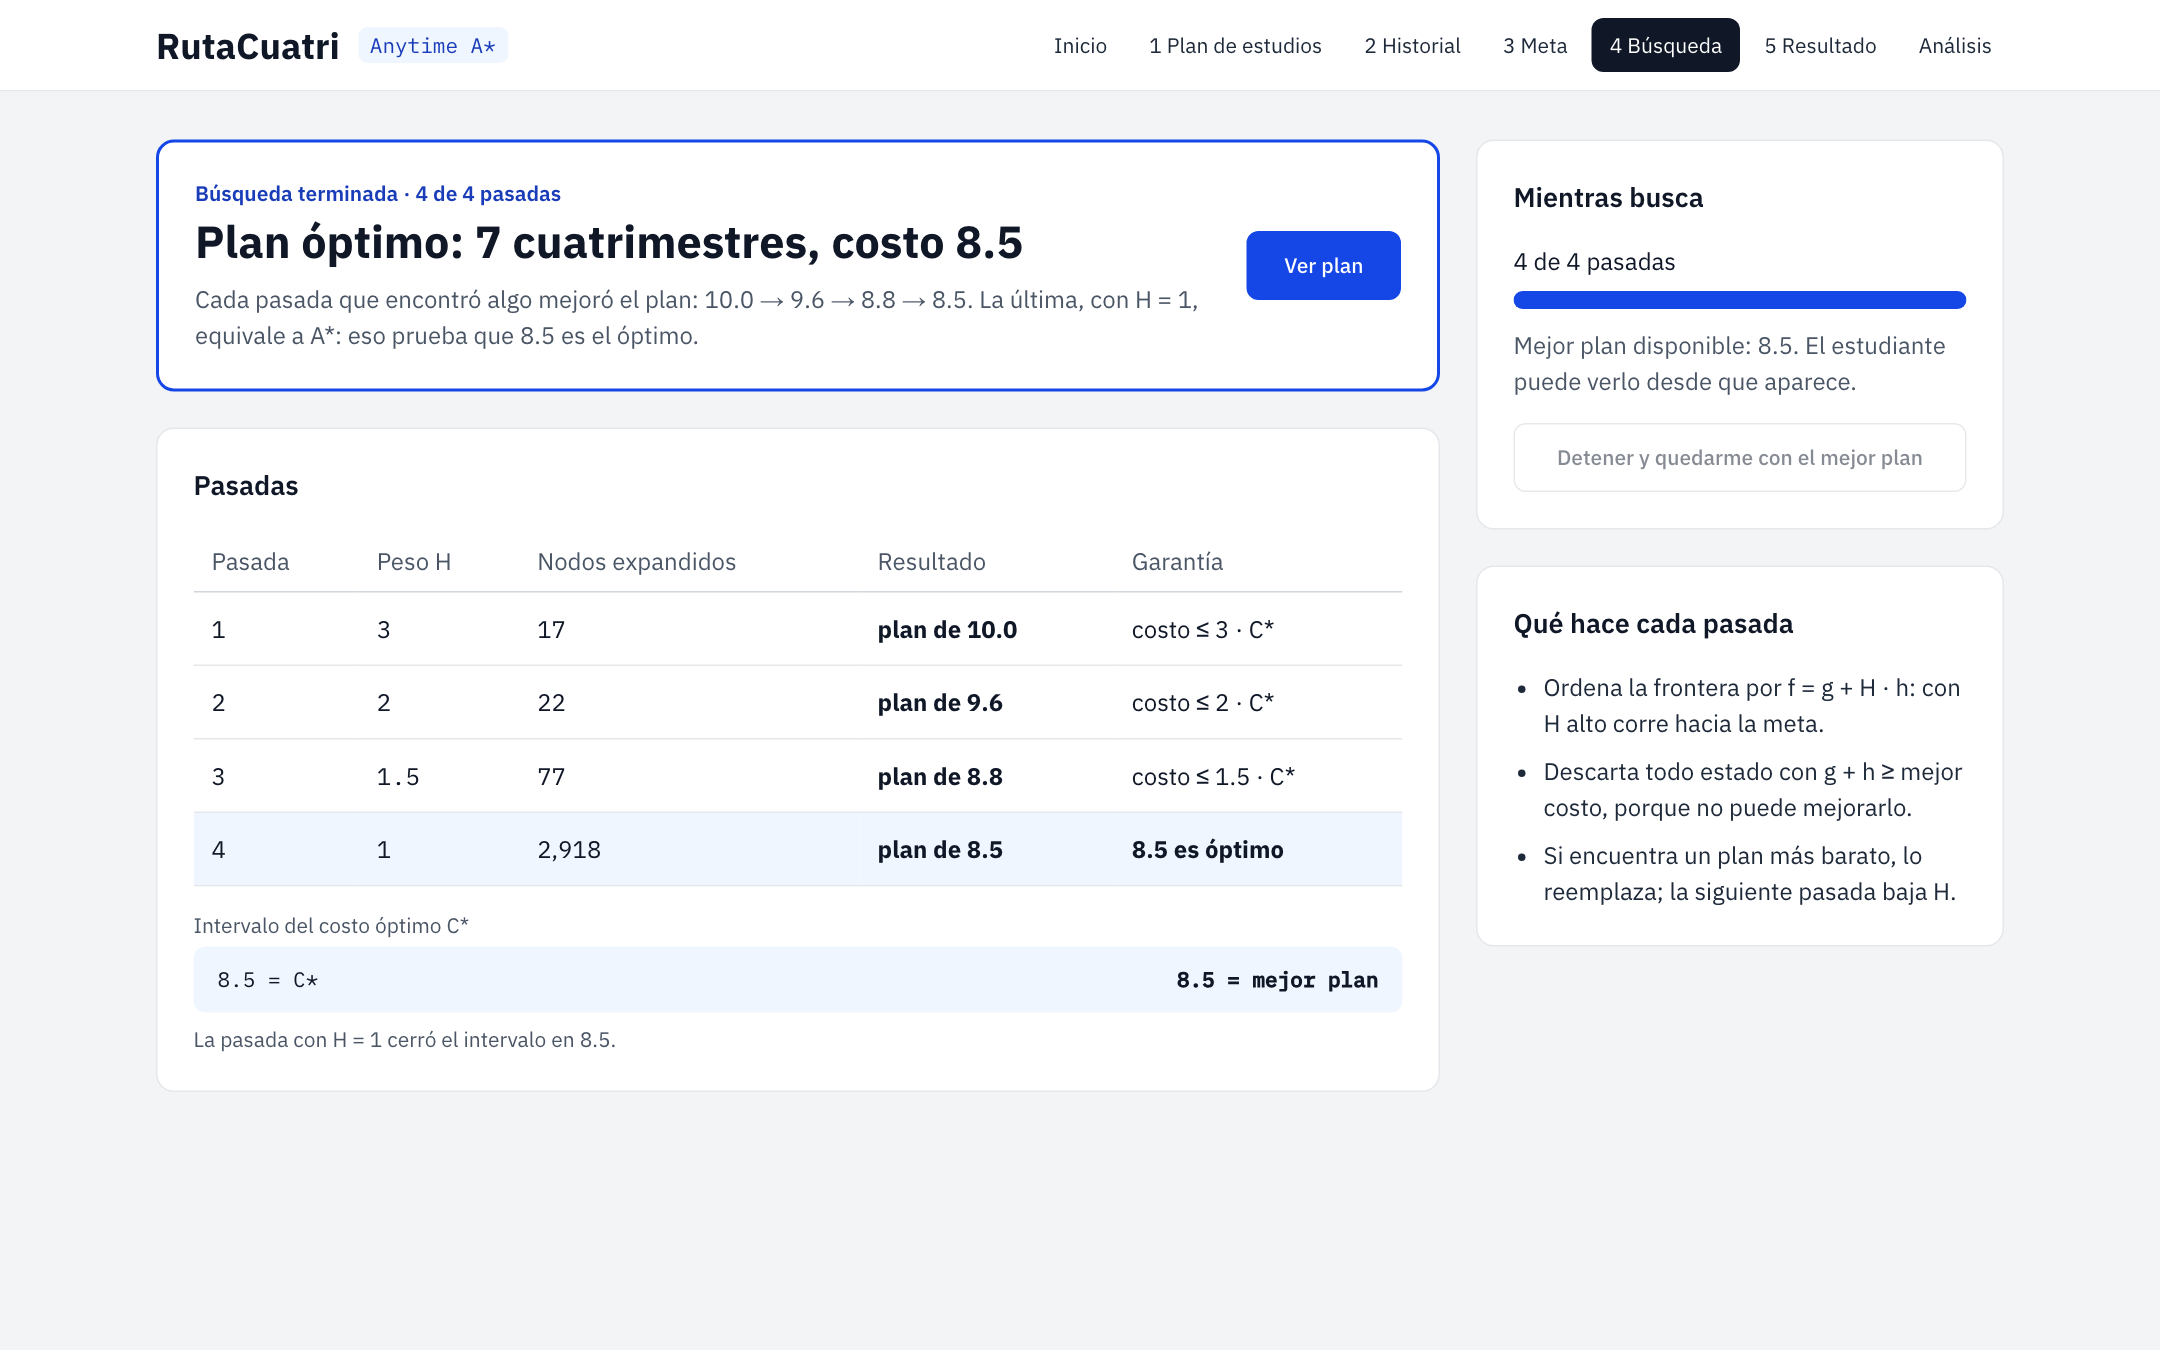
\includegraphics[width=\textwidth,height=0.75\textheight,keepaspectratio]{caso2-busqueda}
    \caption{Caso 2: cada pasada mejora el plan}
    \label{FIG::C2Busqueda}
\end{figure}

\subsection{Comentarios}
Es el caso en que Anytime A* se distingue: el primer plan cuesta 18\% más que el óptimo y llega con menos del 1\% de las expansiones de A*. La pasada final hace el 96\% del trabajo, que es el precio de demostrar el óptimo. El plan muestra que con medio tiempo conviene cargar de más en algunos cuatrimestres: 15 créditos extra cuestan 1.5, menos que los cuatrimestres adicionales que harían falta para no cargar nada.

\section{Caso 3: llegar a la estadía en Redes y Ciberseguridad}

\subsection{Descripción}
Un estudiante de nuevo ingreso de Ingeniería en Redes y Ciberseguridad (IRC) con carga de medio tiempo no quiere todavía la especialidad: quiere saber cuándo puede empezar la estadía. El caso cambia la malla, la meta y el perfil respecto a los anteriores.

\subsection{Estado inicial y meta}
El estado inicial es $(\emptyset, \text{Sep})$ en la malla IRC y la meta es M2, las 23 obligatorias. La cota inicial es $h = \max(\lceil 142/30 \rceil, 5) = 5$, por la cadena IRC03 $\to$ IRC08 $\to$ IRC11 $\to$ IRC16 $\to$ IRC20 (Figura~\ref{FIG::C3Meta}).

\begin{figure}[H]
    \centering
    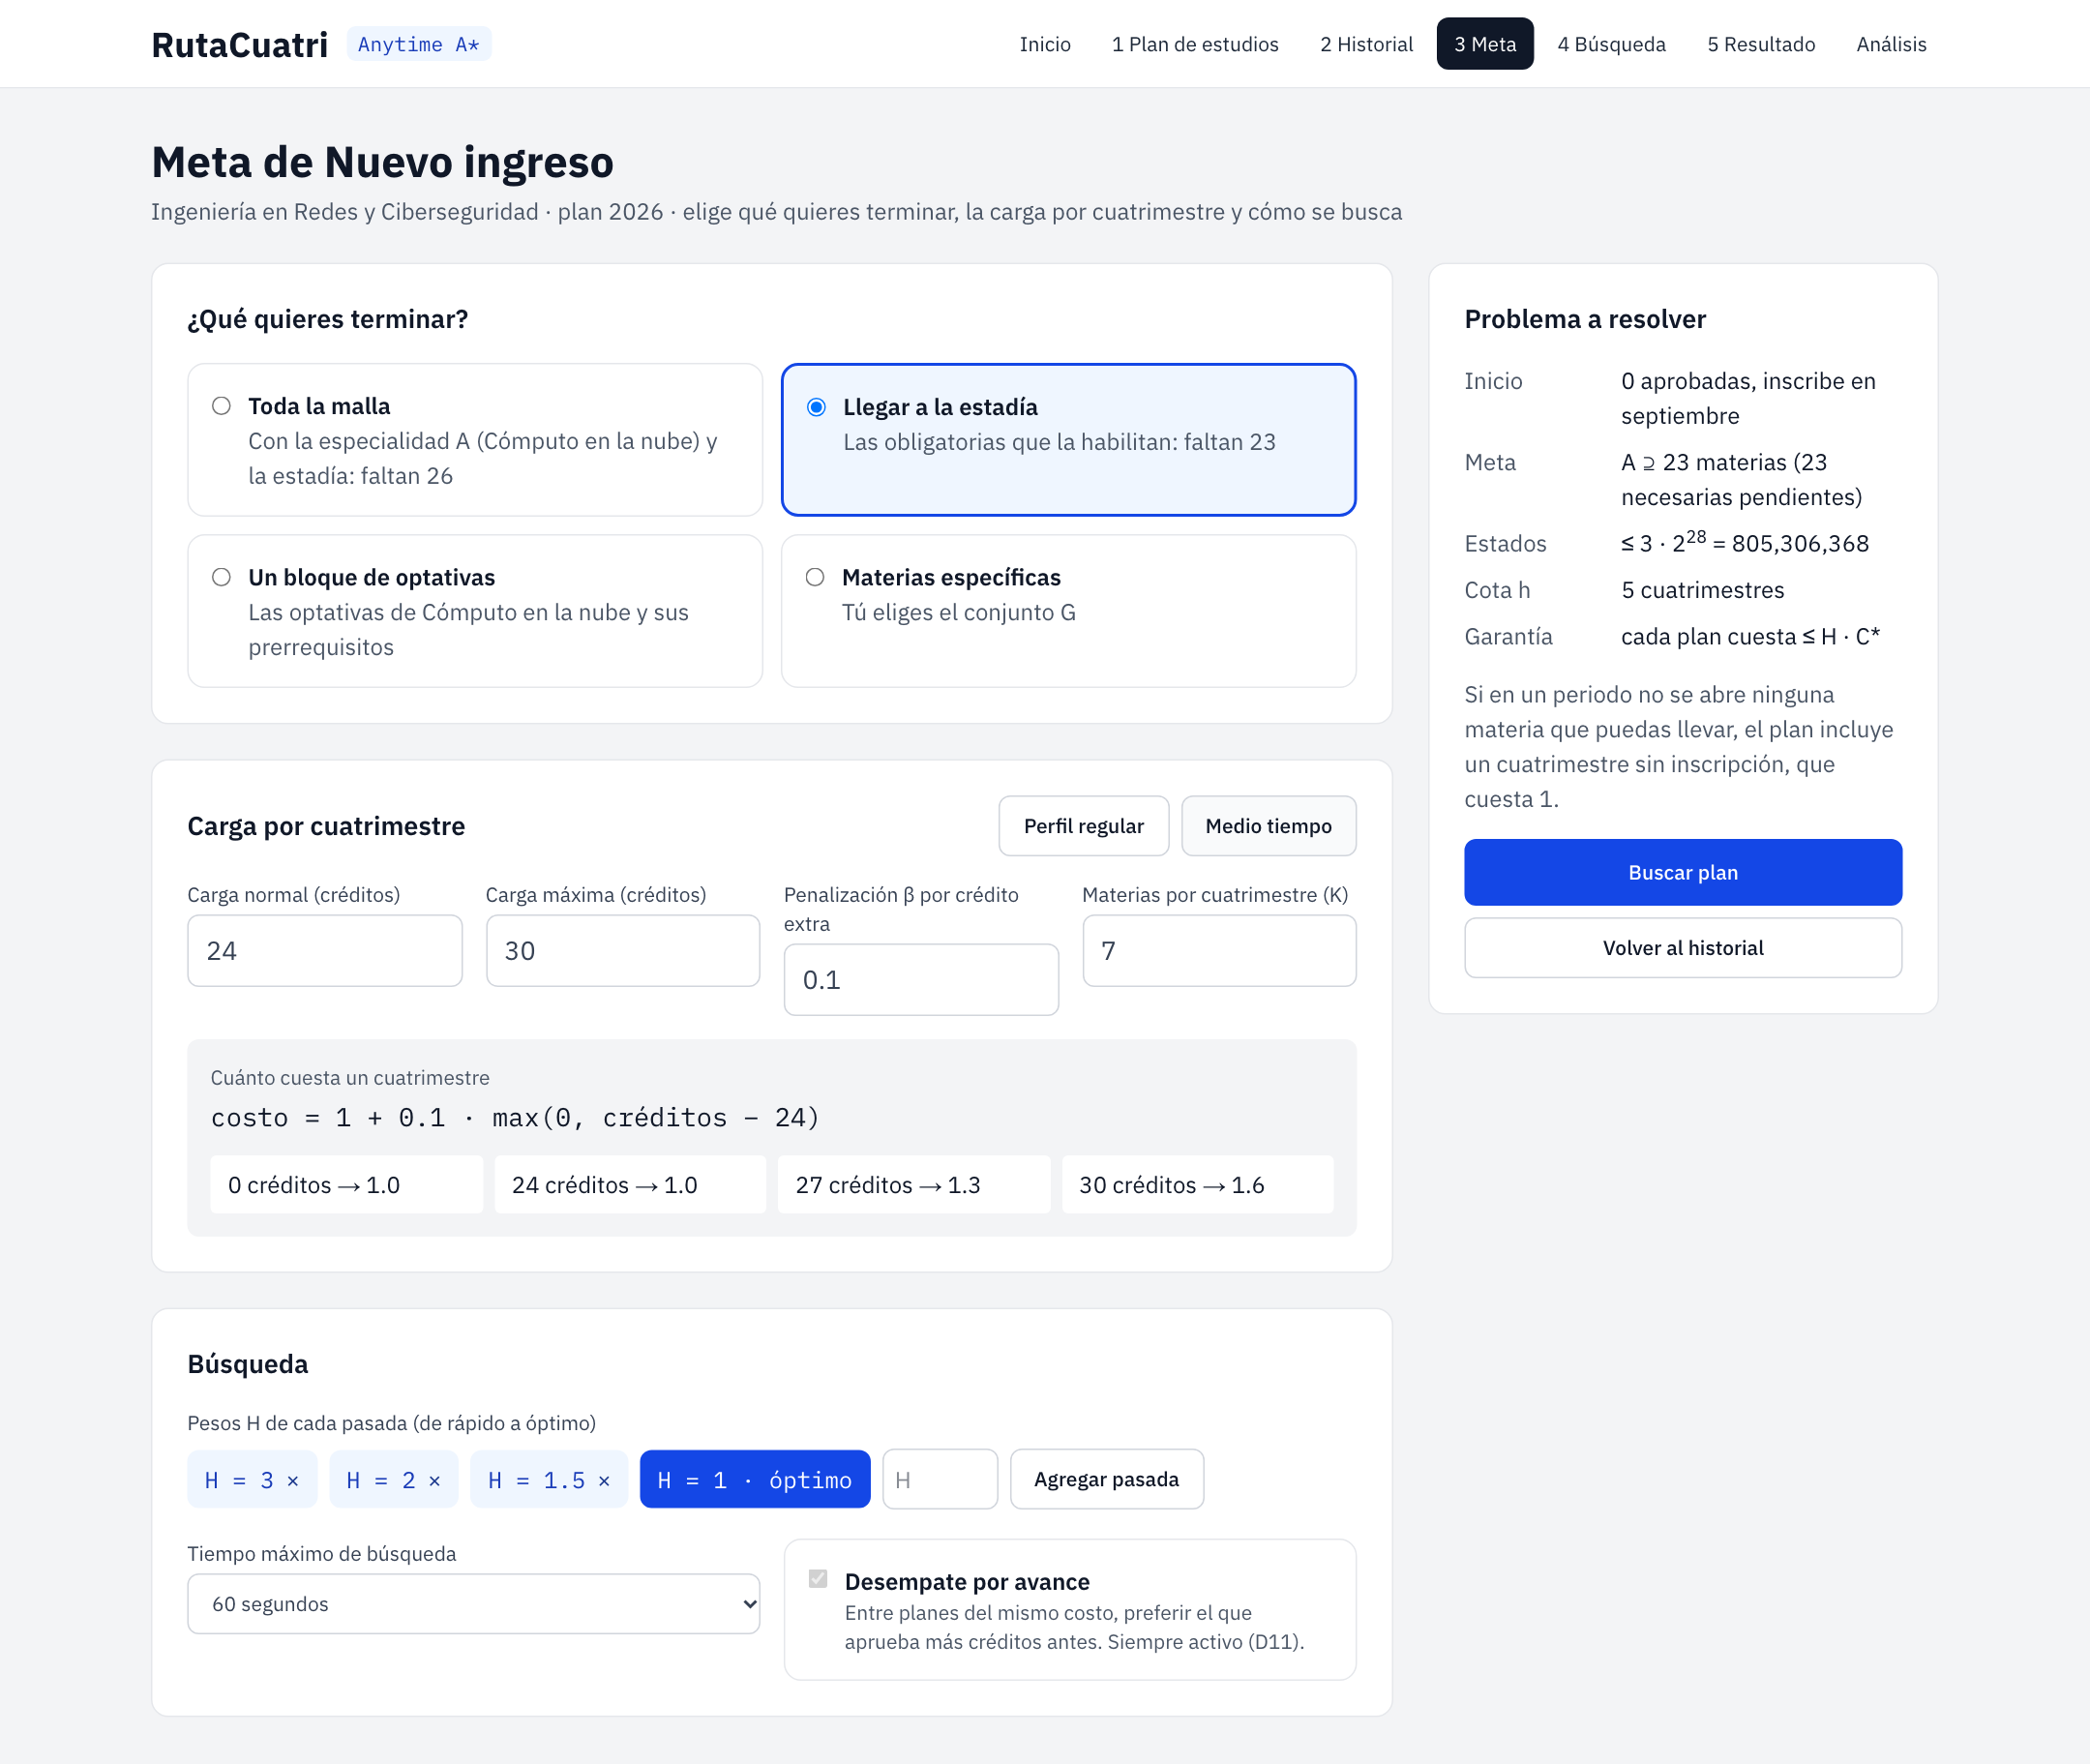
\includegraphics[width=\textwidth,height=0.75\textheight,keepaspectratio]{caso3-meta}
    \caption{Caso 3: meta ``llegar a la estadía'' con medio tiempo}
    \label{FIG::C3Meta}
\end{figure}

\subsection{Solución}
El plan óptimo tiene 6 cuatrimestres y costo 6.1 (Figura~\ref{FIG::C3Resultado}): cinco cuatrimestres sin sobrecarga y uno de 25 créditos, un crédito arriba de la carga normal.

\begin{figure}[H]
    \centering
    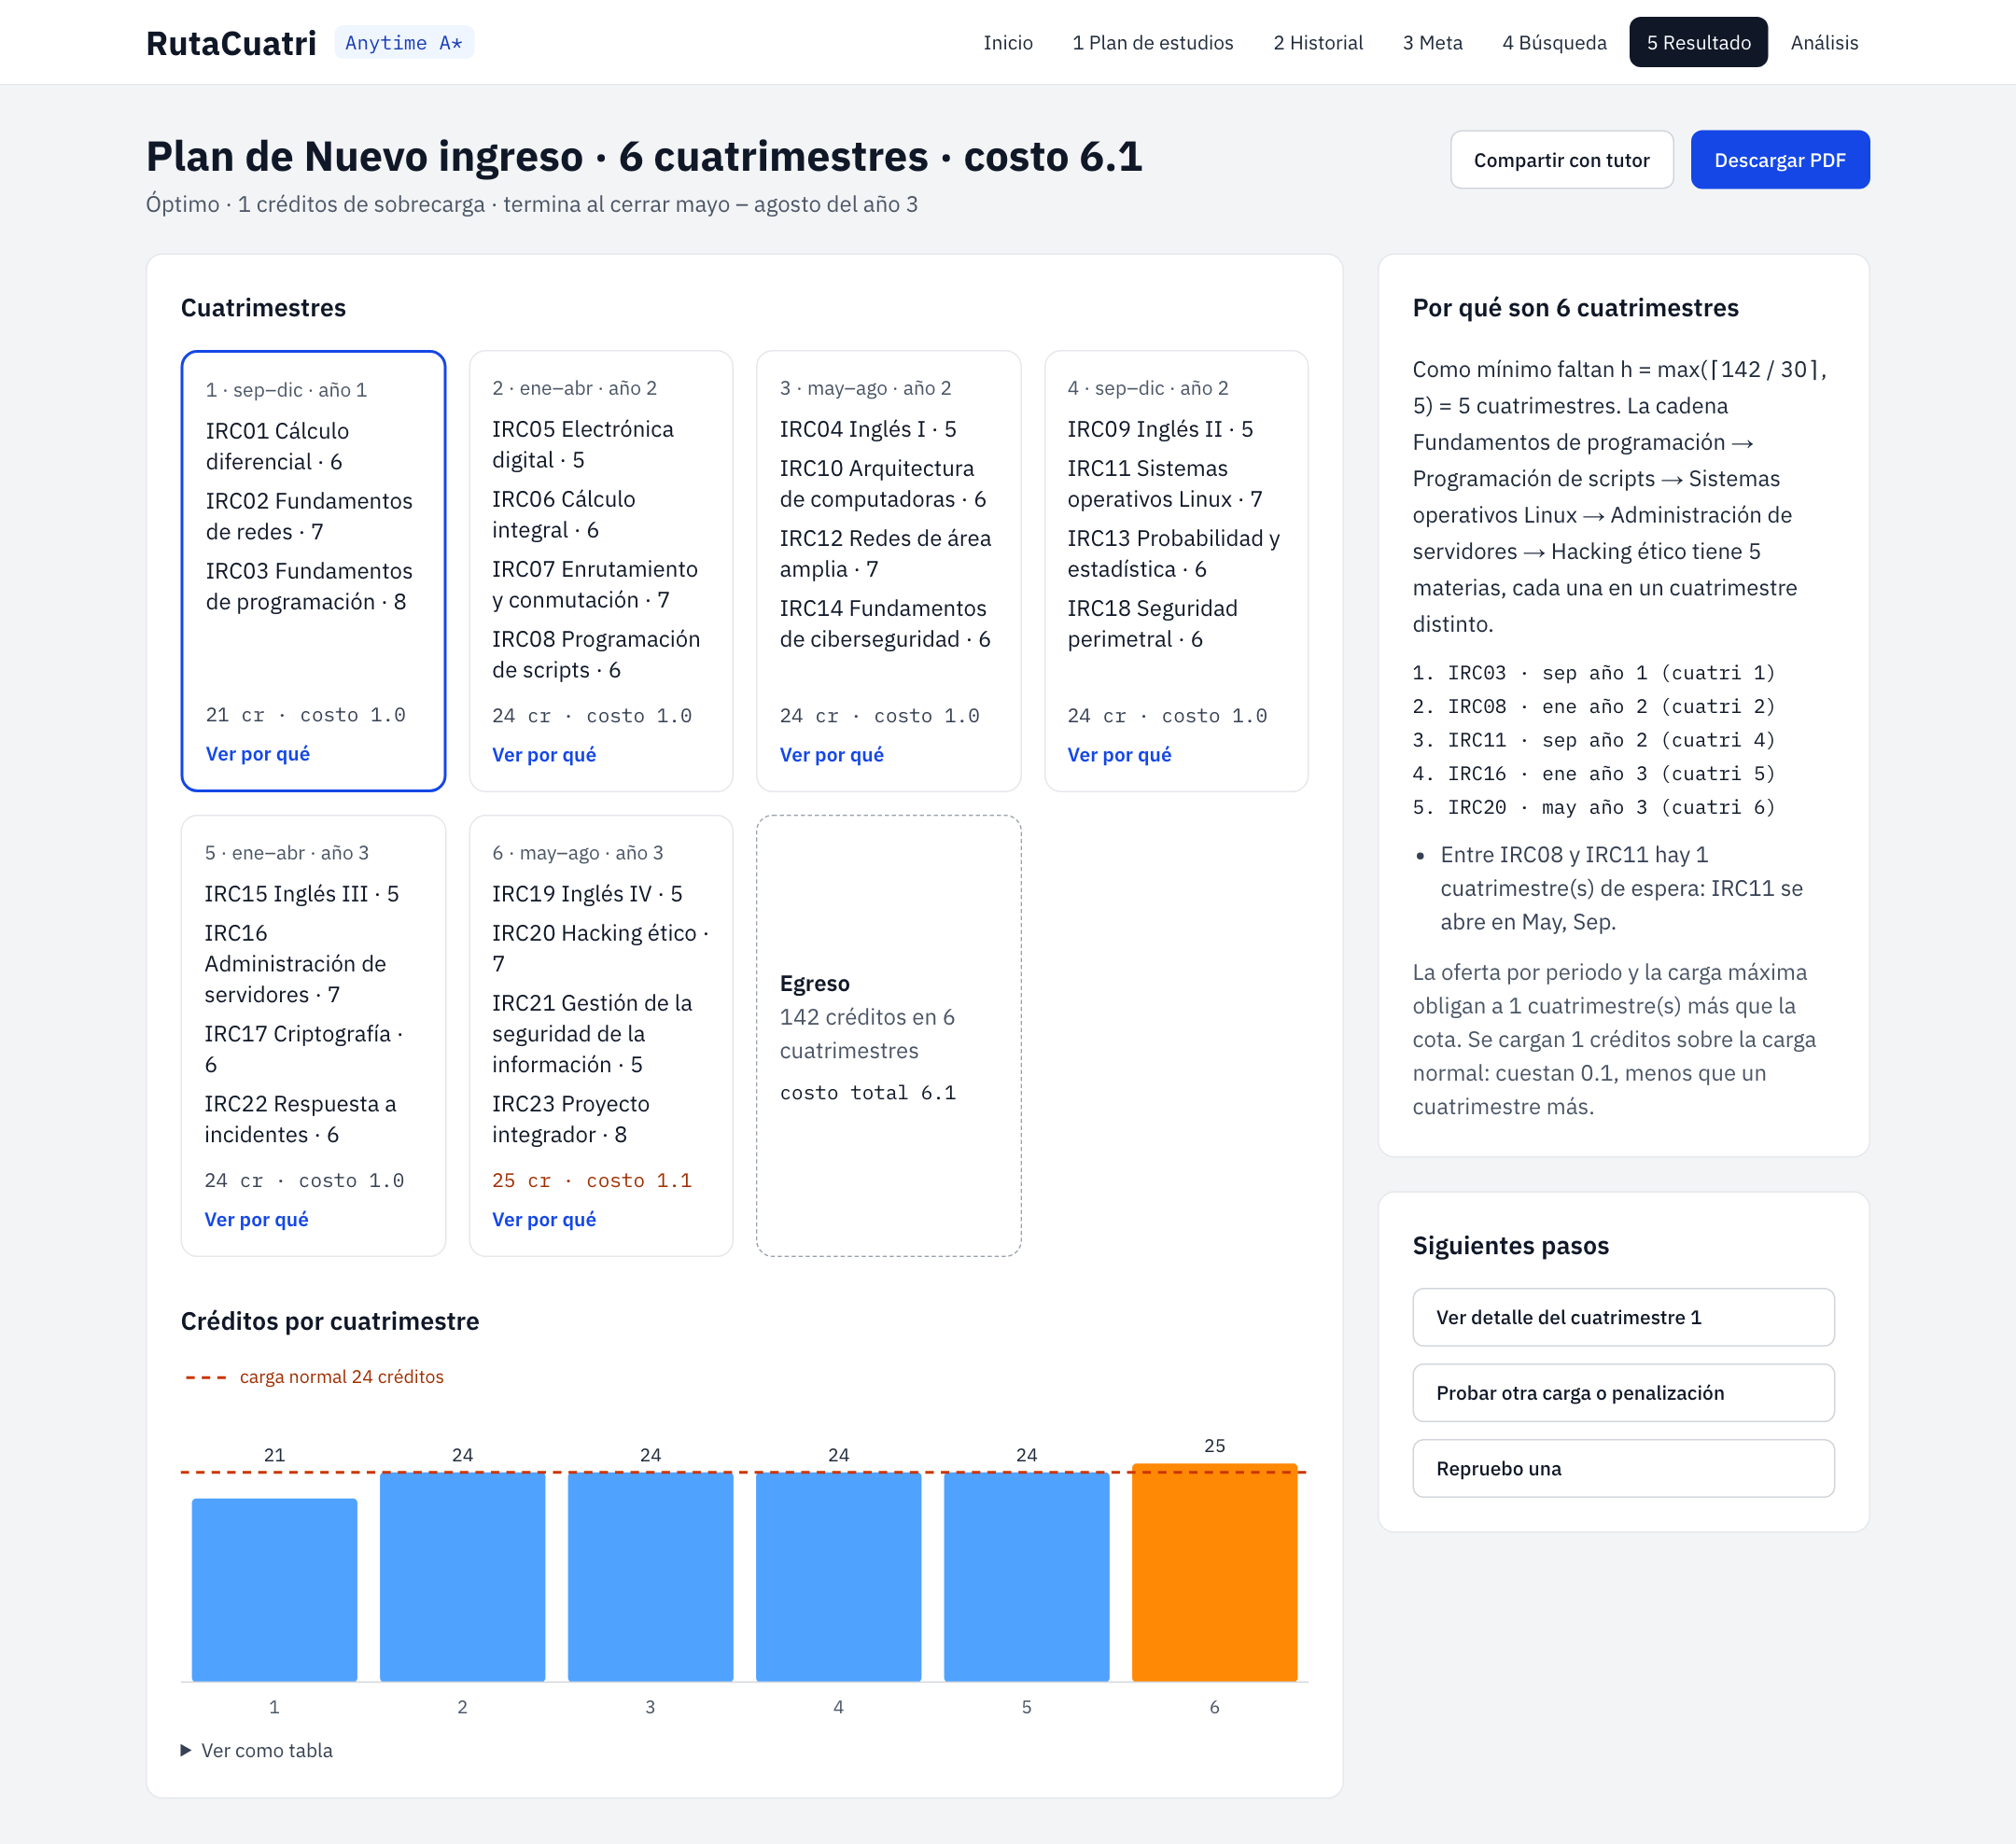
\includegraphics[width=\textwidth,height=0.75\textheight,keepaspectratio]{caso3-resultado}
    \caption{Caso 3: plan óptimo para llegar a la estadía}
    \label{FIG::C3Resultado}
\end{figure}

\subsection{Ejecución}
Las cuatro pasadas vuelven a mejorar el plan: 7.0, 6.8, 6.4 y 6.1, con 6, 10, 7 y 38 expansiones (Figura~\ref{FIG::C3Busqueda}).

\begin{figure}[H]
    \centering
    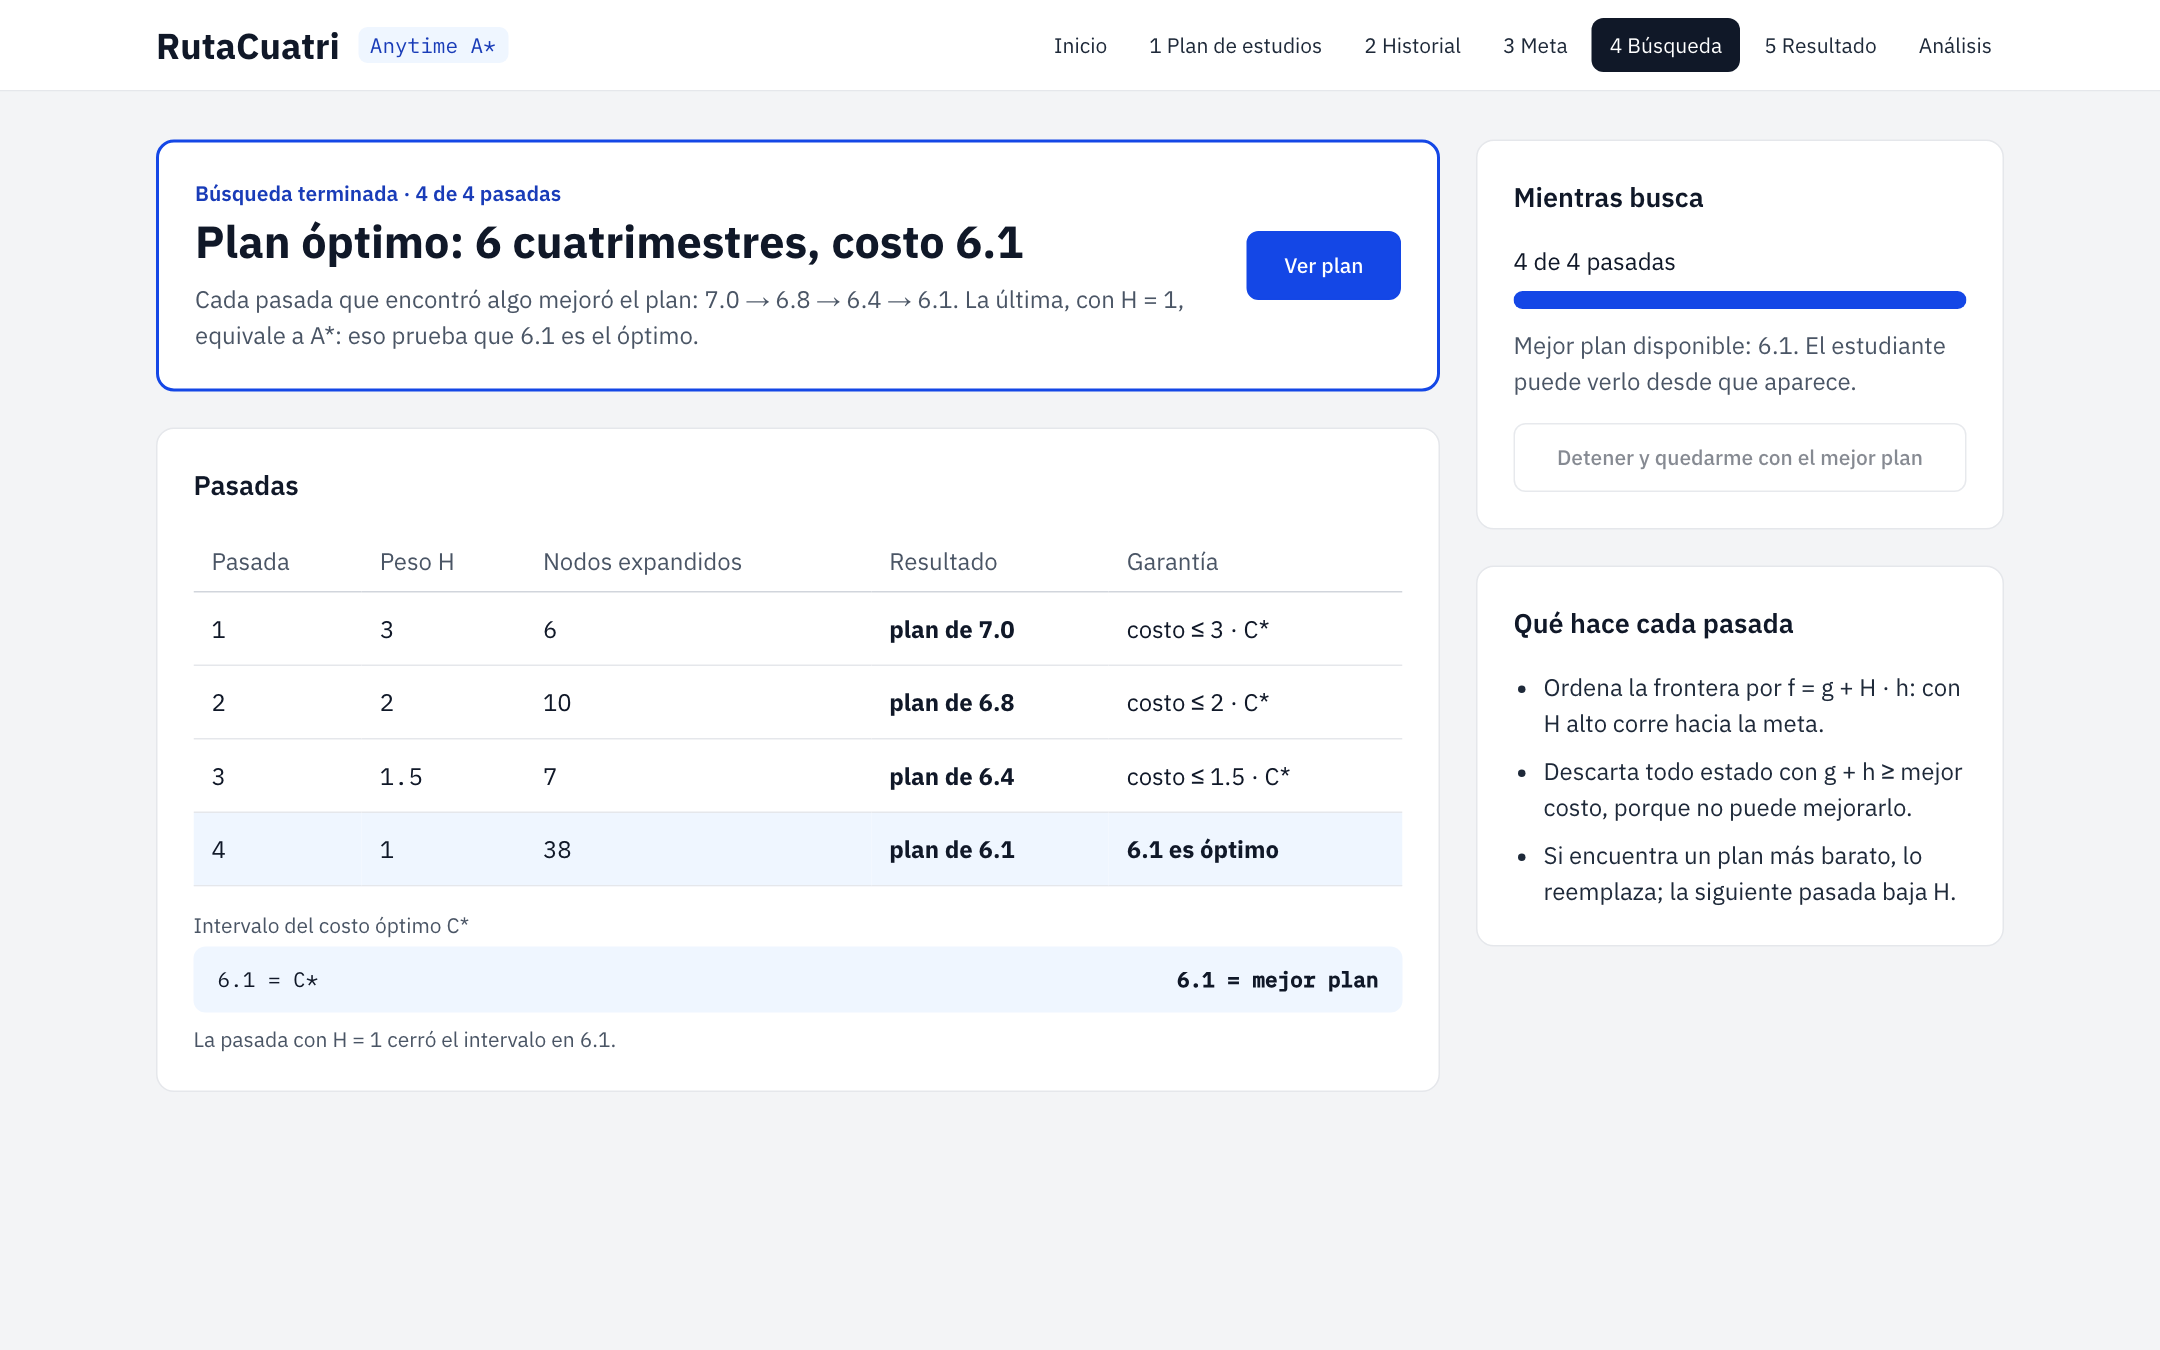
\includegraphics[width=\textwidth,height=0.75\textheight,keepaspectratio]{caso3-busqueda}
    \caption{Caso 3: pasadas de Anytime A*}
    \label{FIG::C3Busqueda}
\end{figure}

\subsection{Comentarios}
El óptimo usa un cuatrimestre más que la cota: la cadena de cinco materias pide 5, pero con 24 créditos de carga normal los 142 créditos no caben sin sobrecarga en 5 cuatrimestres. El plan acepta un solo crédito de sobrecarga, que cuesta 0.1, en lugar de un séptimo cuatrimestre. La pasada con $H = 3$ ya da un plan de 7.0, a 15\% del óptimo.

\section{Caso 4: meta imposible}

\subsection{Descripción}
Se modificó la malla ISW para que Proyecto integrador (ISW23) no se abra en ningún periodo; es el caso especial T03 de las pruebas. Como ISW23 es necesaria para la estadía y la titulación, ningún plan puede cumplir la meta M1.

\subsection{Estado inicial y meta}
El estado inicial es el de nuevo ingreso, $(\emptyset, \text{Sep})$, y la meta es M1. La Figura~\ref{FIG::C4Malla} muestra la tabla de materias con ISW23 marcada ``Sin oferta''.

\begin{figure}[H]
    \centering
    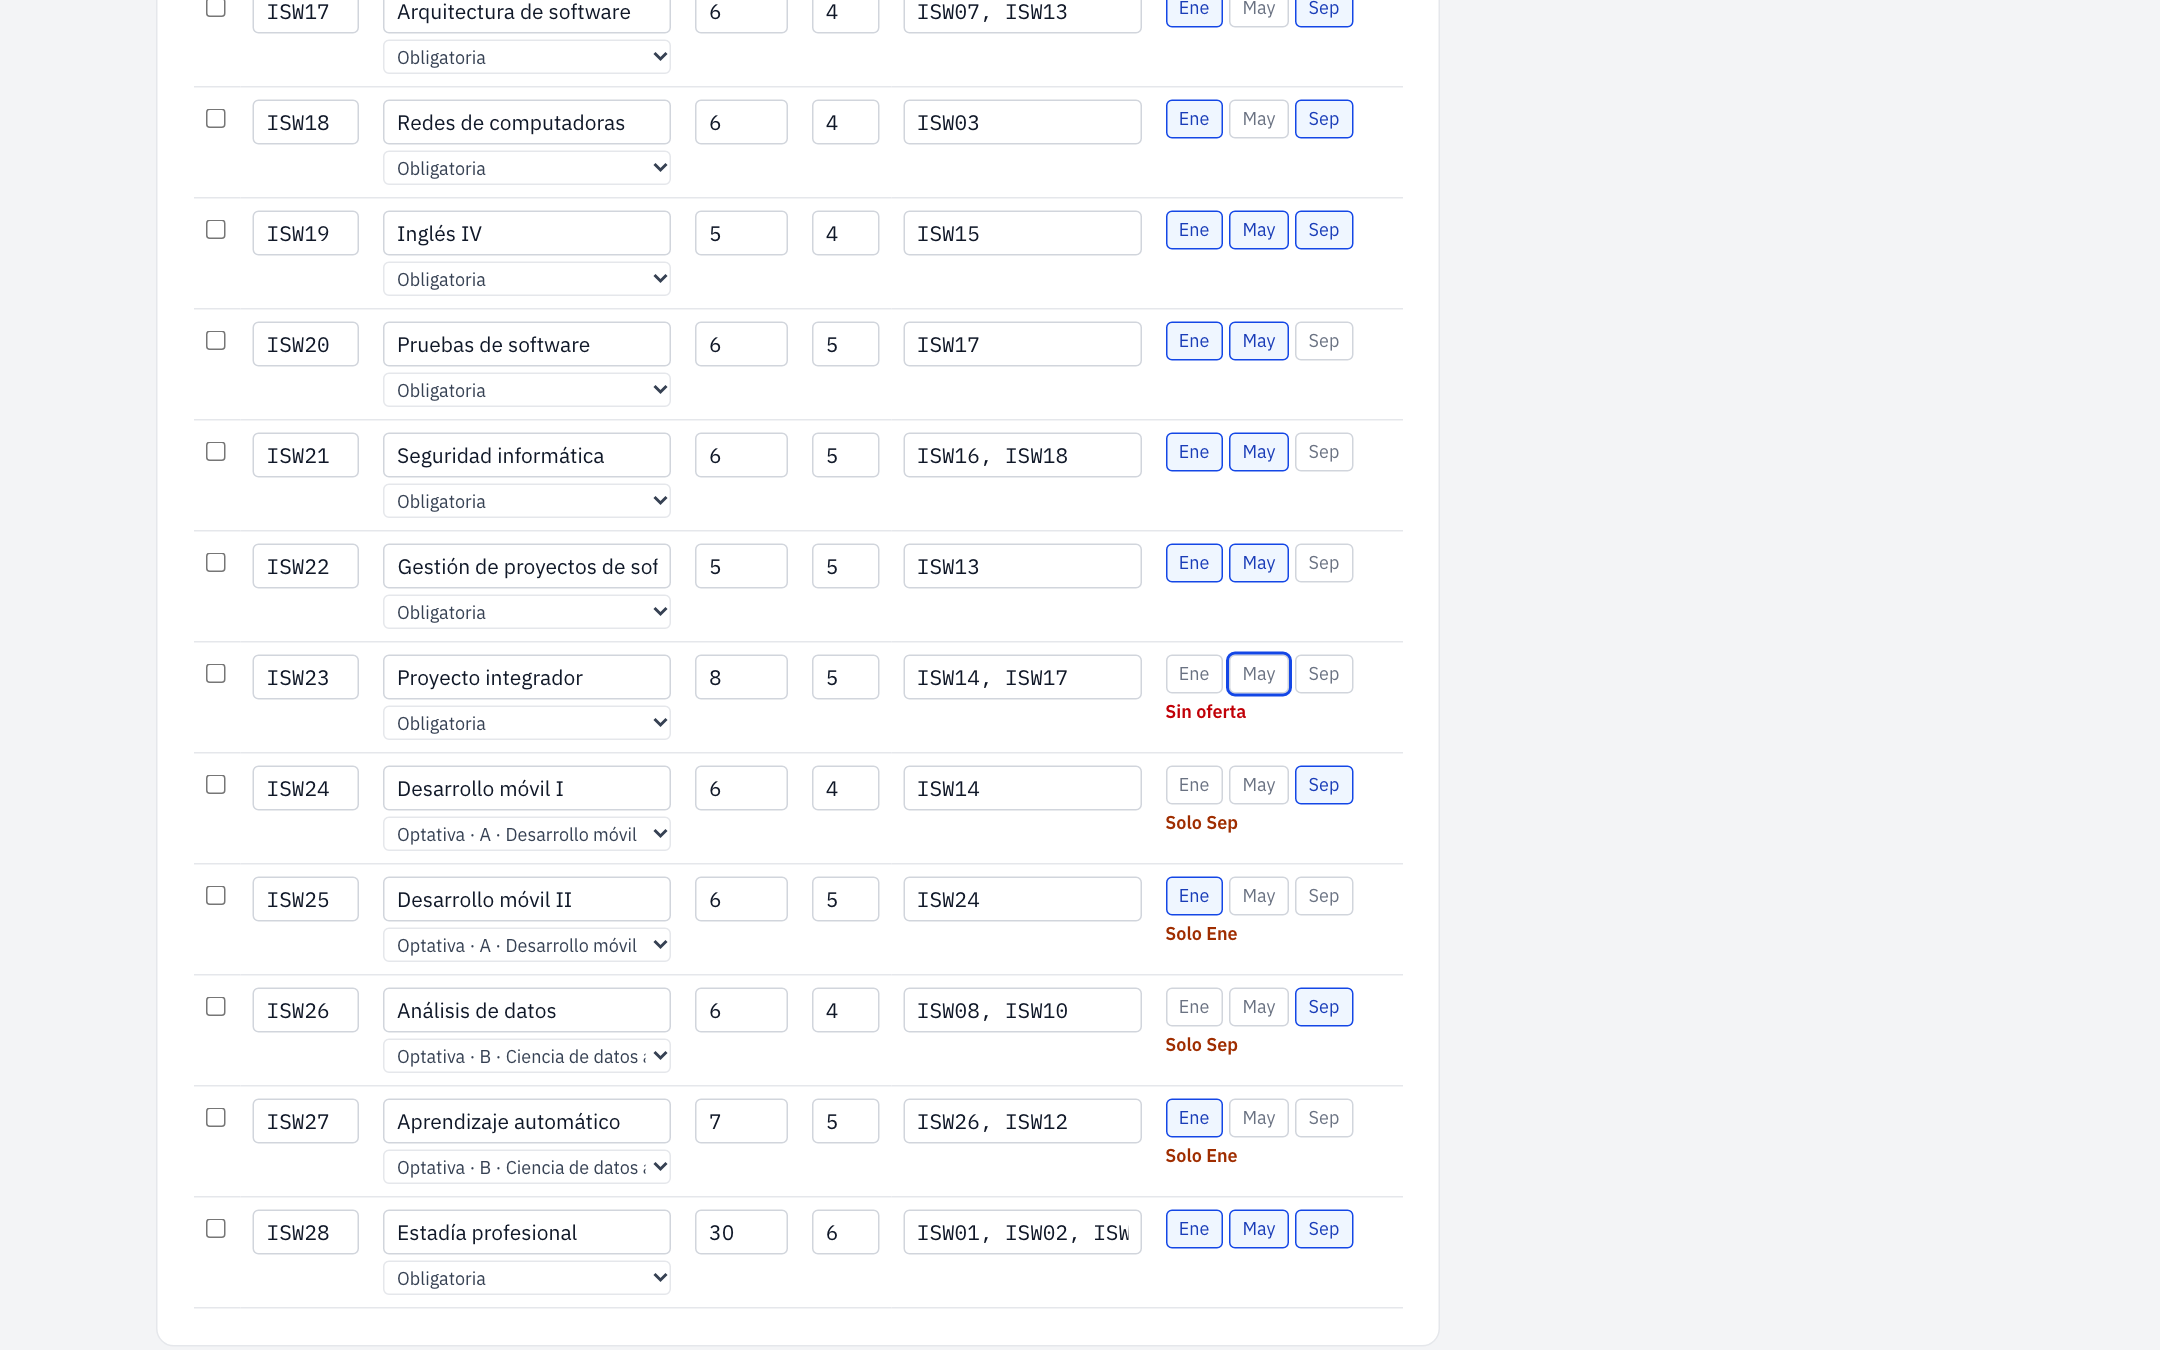
\includegraphics[width=\textwidth,height=0.75\textheight,keepaspectratio]{caso4-malla}
    \caption{Caso 4: ISW23 sin oferta en el plan de estudios}
    \label{FIG::C4Malla}
\end{figure}

\subsection{Solución}
Al presionar ``Buscar plan'', la validación detecta que una materia necesaria no se abre en ningún periodo y la interfaz va directo a la pantalla ``Sin plan posible'' sin ejecutar la búsqueda (Figura~\ref{FIG::C4SinPlan}). La pantalla muestra la causa (la materia, sus prerrequisitos y su oferta) y tres opciones: planear sin esa materia, solicitar que se abra (con un enlace para revisar su oferta en el plan de estudios) o cambiar la meta.

\begin{figure}[H]
    \centering
    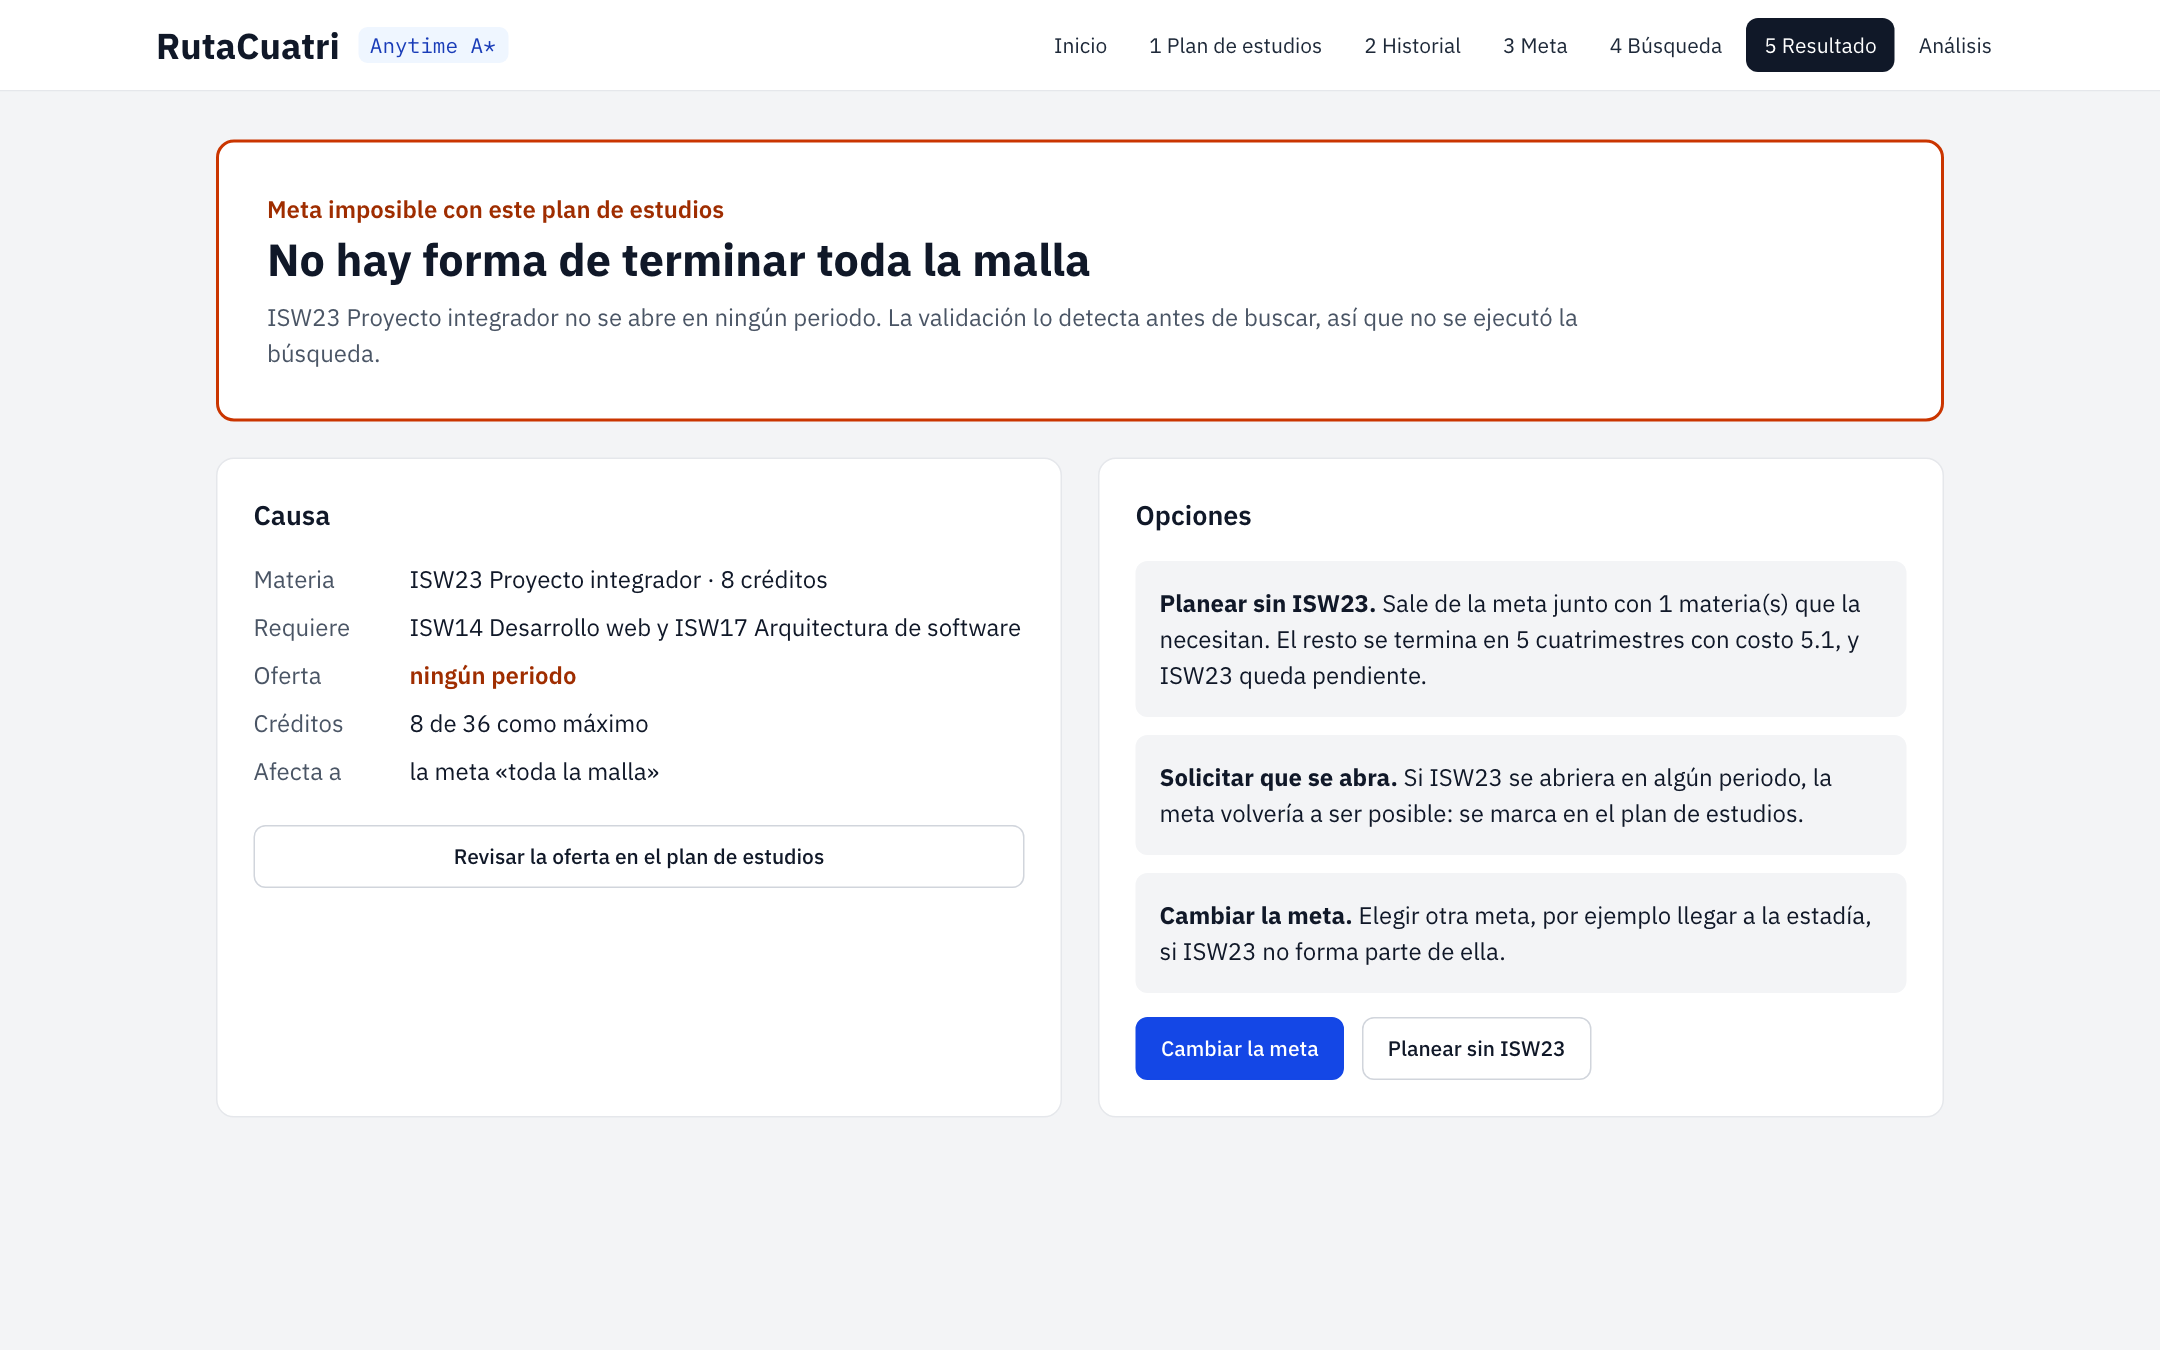
\includegraphics[width=\textwidth,height=0.75\textheight,keepaspectratio]{caso4-sin-plan}
    \caption{Caso 4: pantalla ``Sin plan posible''}
    \label{FIG::C4SinPlan}
\end{figure}

\subsection{Ejecución}
No hay pasadas: la búsqueda nunca empieza. La opción ``Planear sin ISW23'' quita de la meta a ISW23 y a la estadía, que la necesita, y calcula con A* el plan del resto: 24 materias en 5 cuatrimestres con costo 5.1.

\subsection{Comentarios}
Validar antes de buscar evita una búsqueda inútil: sin la validación, la búsqueda tendría que agotar todo el espacio alcanzable para concluir que no hay plan. Como las reglas de la validación garantizan que, si pasan, siempre existe un plan, la pantalla ``Sin plan posible'' sale solo de la validación.

\section{Experimentos}
Los cuatro experimentos se corren con el script \texttt{scripts/experimento.ts}, que usa el mismo motor en Node y escribe un archivo CSV por experimento. Cada corrida se repite 5 veces y se reporta la mediana del tiempo; los costos y las expansiones no cambian entre repeticiones. Una corrida se corta a los 60 s, pero ninguna llegó a ese límite.

\subsection{Experimento A: primer plan y óptimo}
Se corrió Anytime A* en los 72 escenarios. En los 72 el costo final coincide con el óptimo esperado y cada pasada cumple $\text{costo} \leq H \cdot C^*$. En 52 de los 72 escenarios la primera pasada ya da el plan óptimo (27 de 36 con el perfil regular y 25 de 36 con medio tiempo). El peor primer plan es el de Daniel Ortega en ICD con la meta M1: 6.1 contra un óptimo de 4.3, es decir, 1.42 veces el óptimo, muy por debajo de la garantía de 3. La mediana del tiempo hasta el primer plan es de 0.04 ms y la del tiempo total de 0.08 ms; el escenario más largo es el Caso 2, con 38.6 ms.

La Figura~\ref{FIG::ExpA} muestra el costo del mejor plan contra las expansiones acumuladas en el Caso 2: el plan baja de 10.0 a 8.5 y casi todo el trabajo está en la última pasada.

\begin{figure}[H]
    \centering
    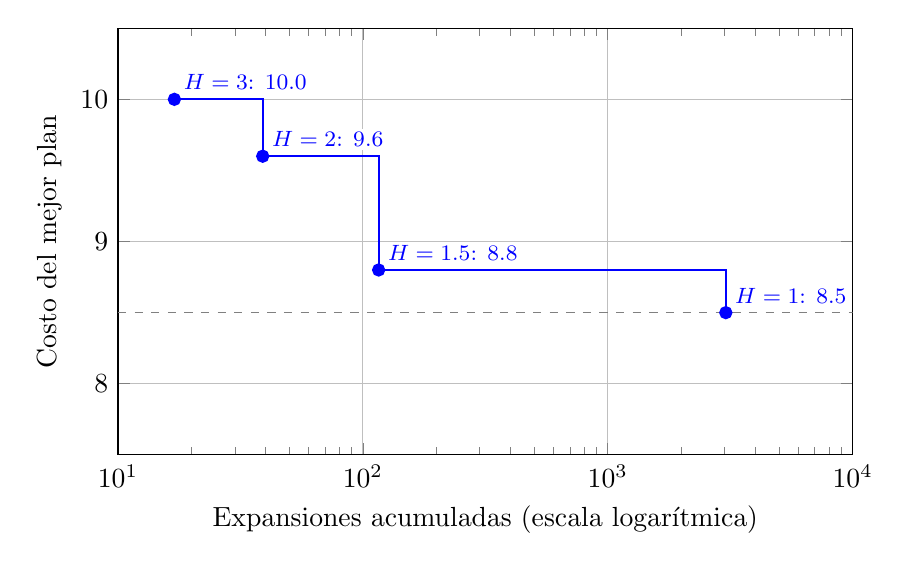
\begin{tikzpicture}
        \begin{semilogxaxis}[
            width=0.9\textwidth, height=7cm,
            xlabel={Expansiones acumuladas (escala logarítmica)},
            ylabel={Costo del mejor plan},
            ymin=7.5, ymax=10.5,
            xmin=10, xmax=10000,
            grid=major,
        ]
            \addplot[const plot, thick, blue, mark=*,
                nodes near coords, point meta=explicit symbolic,
                every node near coord/.append style={font=\footnotesize, anchor=south west, fill=white, inner sep=1pt, xshift=2pt, yshift=2pt}] coordinates {
                (17,10.0)[$H=3$: 10.0]
                (39,9.6)[$H=2$: 9.6]
                (116,8.8)[$H=1.5$: 8.8]
                (3034,8.5)[$H=1$: 8.5]
            };
            \addplot[dashed, gray] coordinates {(10,8.5) (10000,8.5)};
        \end{semilogxaxis}
    \end{tikzpicture}
    \caption{Experimento A: costo contra expansiones acumuladas de Anytime A*, ISW-E1, meta M1, medio tiempo. La línea punteada es el óptimo.}
    \label{FIG::ExpA}
\end{figure}

\subsection{Experimento B: comparación de métodos}
Se compararon Anytime A*, A*, Weighted A* con $H = 2$ y Costo Uniforme en los 24 escenarios con meta M1. La Tabla~\ref{TAB::ExpB} y la Figura~\ref{FIG::ExpB} resumen los resultados.

\begin{table}[H]
  \begin{center}
    \caption{Experimento B: 24 escenarios con meta M1}
    \label{TAB::ExpB}
    \begin{tabular}{|| l | r | c | r ||}
        \hline
        Método & Expansiones totales & Óptimos & Primer plan, medio tiempo \\ [0.5ex]
        \hline\hline
        Anytime A* & 7,197 & 24 / 24 & 0.05 ms \\
        \hline
        A* & 5,523 & 24 / 24 & 0.23 ms \\
        \hline
        Weighted A* ($H = 2$) & 270 & 11 / 24 & 0.07 ms \\
        \hline
        Costo Uniforme & 10,452 & 24 / 24 & 0.17 ms \\
        \hline
    \end{tabular}
  \end{center}
\end{table}

\begin{figure}[H]
    \centering
    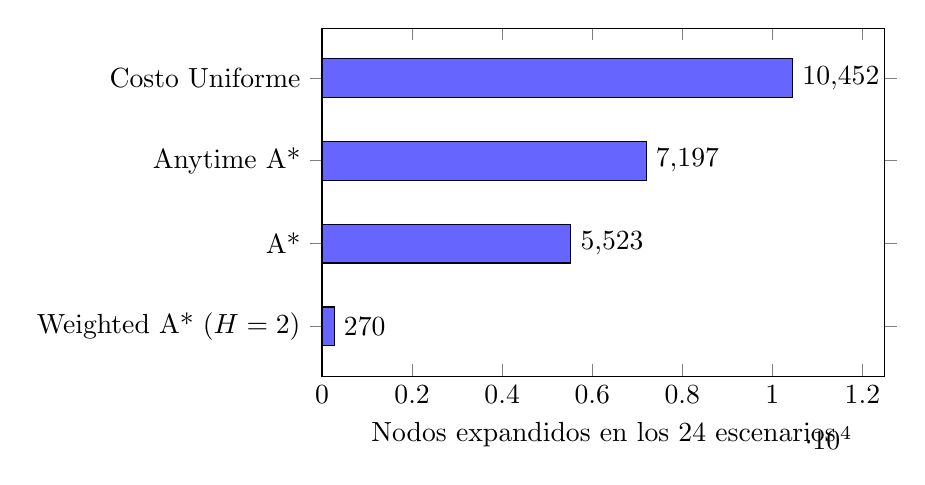
\begin{tikzpicture}
        \begin{axis}[
            xbar, width=0.72\textwidth, height=6cm,
            xlabel={Nodos expandidos en los 24 escenarios},
            ytick={1,2,3,4},
            yticklabels={Weighted A* ($H=2$), A*, Anytime A*, Costo Uniforme},
            xmin=0, xmax=12500,
            nodes near coords,
            nodes near coords align={horizontal},
            bar width=14pt,
            enlarge y limits=0.2,
        ]
            \addplot[fill=blue!60] coordinates {(270,1) (5523,2) (7197,3) (10452,4)};
        \end{axis}
    \end{tikzpicture}
    \caption{Experimento B: expansiones por método}
    \label{FIG::ExpB}
\end{figure}

Costo Uniforme es óptimo pero, sin heurística, expande casi el doble que A*. Weighted A* con $H = 2$ expande muy poco pero solo da el óptimo en 11 de 24 casos. Anytime A* expande 30\% más que A* porque repite la búsqueda en cada pasada, y a cambio entrega un plan desde la primera pasada y siempre llega al óptimo.

\subsection{Experimento C: reglas de poda}
Se corrió A* con y sin las reglas de generación de sucesores (solo materias necesarias, poda por dominancia y cuatrimestre vacío solo si no hay nada) para los estudiantes E1 y E3, con la meta M1 y medio tiempo. La Tabla~\ref{TAB::ExpC} muestra que el costo es el mismo en los seis casos y que las reglas reducen las expansiones entre 2.3 y 18.9 veces.

\begin{table}[H]
  \begin{center}
    \caption{Experimento C: nodos expandidos por A* con y sin las reglas}
    \label{TAB::ExpC}
    \begin{tabular}{|| l | c | r | r | r ||}
        \hline
        Estudiante & Costo & Sin reglas & Con reglas & Ahorro \\ [0.5ex]
        \hline\hline
        ISW-E1 & 8.5 & 8,644 & 2,918 & 3.0 \\
        \hline
        ISW-E3 & 6.6 & 2,453 & 1,084 & 2.3 \\
        \hline
        IRC-E1 & 8.6 & 1,423 & 393 & 3.6 \\
        \hline
        IRC-E3 & 7.6 & 450 & 33 & 13.6 \\
        \hline
        ICD-E1 & 8.5 & 2,807 & 574 & 4.9 \\
        \hline
        ICD-E3 & 7.6 & 284 & 15 & 18.9 \\
        \hline
    \end{tabular}
  \end{center}
\end{table}

\subsection{Experimento D: qué parámetro decide el egreso}
Se corrió A* para el nuevo ingreso de ISW con la meta M1, cambiando un solo parámetro del perfil regular cada vez (Tabla~\ref{TAB::ExpD}).

\begin{table}[H]
  \begin{center}
    \caption{Experimento D: sensibilidad para ISW-E1, meta M1}
    \label{TAB::ExpD}
    \begin{tabular}{|| l | c | c | c ||}
        \hline
        Cambio sobre el perfil regular & Costo & Cuatrimestres & Créditos de sobrecarga \\ [0.5ex]
        \hline\hline
        Ninguno & 6.4 & 6 & 4 \\
        \hline
        $\beta = 0.05$ & 6.2 & 6 & 4 \\
        \hline
        $\beta = 0.2$ & 6.8 & 6 & 4 \\
        \hline
        $\beta = 0.5$ & 7.0 & 7 & 0 \\
        \hline
        $C_{norm} = 24$ & 8.5 & 7 & 15 \\
        \hline
        $C_{norm} = 27$ & 7.4 & 7 & 4 \\
        \hline
        $C_{norm} = 33$ & 6.0 & 6 & 0 \\
        \hline
        $C_{max} = 30$ & 7.0 & 7 & 0 \\
        \hline
        $C_{max} = 33$ o $40$ & 6.4 & 6 & 4 \\
        \hline
        $K = 5$ o $6$ & 6.4 & 6 & 4 \\
        \hline
    \end{tabular}
  \end{center}
\end{table}

La carga normal es la que más mueve el egreso: con $C_{norm} = 24$ el plan pasa a 7 cuatrimestres y aun así carga 15 créditos de más. Subir la carga máxima arriba de 33 no adelanta nada, porque lo que manda es la cadena de seriación. Con $\beta = 0.5$ conviene un séptimo cuatrimestre antes que cargar de más. Los doce valores coinciden con los de la implementación de referencia. La pantalla de análisis repite este experimento para cualquier escenario (Anexo~\ref{ANX::Analisis}).
